\documentclass[10pt,twoside,cucitura,classica,english,openany]{toptesi}

\usepackage{hyperref}
\hypersetup{%
  pdfpagemode={UseOutlines},
  bookmarksopen,
  pdfstartview={FitH},
  colorlinks,
  linkcolor={blue},
  citecolor={red},
  urlcolor={blue}
}
\usepackage[latin1]{inputenc}
\usepackage[T1]{fontenc}\usepackage{lmodern}
\usepackage{layaureo}
\usepackage{amsmath}
\usepackage{mathtools}
\usepackage{amssymb}
\usepackage{placeins}
\usepackage[titletoc]{appendix}
\usepackage[acronym]{glossaries}
\usepackage[font=footnotesize]{caption}
\usepackage[font=footnotesize]{subcaption}
\usepackage[style=numeric, sorting=none, backend=biber]{biblatex}

\makeglossaries

% To change the bullet type of itemize environment
\def\labelitemi{--}

\addbibresource{references.bib}

\bibliography{bibliography}

\ateneo{Stockholm University}
\facolta{Department of Physics}

\titolo{Search for in Mono-jet Final States with the ATLAS Experiment}

\TesiDiLaurea{Licensiate Thesis}

\CorsoDiLaureaIn{Doctoral Studies in }
\corsodilaurea{Physics}

\CandidateName{Candidate:}
\candidato{Gabriele \textsc{Bertoli}}
\AdvisorName{Advisor:}
\relatore{dott.~Christophe \textsc{Clement}}
\CoAdvisorName{Co-Supervisor}
\secondorelatore{dott.~David \textsc{Milstead}}
\sedutadilaurea{December 2015}
\sedutadilaurea{\textsc{December 12,} 2015}
\logosede{logo}

\newtheorem{osservazione}{Osservazione}
\ExtendCaptions{english}{Abstract}{Acknowledgments}

\graphicspath{{images/}}

\begin{document}\errorcontextlines=9

\numberwithin{equation}{section}

\newcommand*{\parder}[2]{\displaystyle\frac{\partial #1}{\partial #2}}
\newcommand*{\ud}{\mathrm{d}}
\newcommand*{\er}{e_{R}}
\newcommand*{\el}{e_{L}}
\newcommand*{\eplus}{e^{+}}
\newcommand*{\eminus}{e^{-}}
\newcommand*{\vect}[1]{\overrightarrow{#1}}
\newcommand*{\bra}[1]{\langle #1|}
\newcommand*{\ket}[1]{|#1\rangle}
\newcommand*{\MET}{\mbox{$E\kern-0.50em\raise0.10ex\hbox{/}_{T}$}}
\newcommand*{\met}{E_\mathrm{\, T}^\mathrm{\, miss}}
\newcommand*{\et}{E_\mathrm{\, T}}
\newcommand*{\pt}{p_\mathrm{\, T}}
\newcommand*{\ifb}{\mbox{fb$^{-1}$}}
\newcommand*{\zee}{Z \to e e}
%%% Local Variables:
%%% mode: latex
%%% TeX-master: "main"
%%% End:


\english

\cleardoublepage

% \expandafter\ifx\csname StileTrieste\endcsname\relax
\frontespizio
% \else
\paginavuota
\begin{dedica}
\end{dedica}
% \tomo \fi

\ringraziamenti

\tablespagetrue\figurespagetrue \indici

% \expandafter\ifx\csname StileTrieste\endcsname\relax \else
\begin{citazioni}
  \textit{Si sta,\\come d'autunno,\\sugli alberi,\\le foglie }

  [\textsc{G.~Ungaretti}, Soldati]
\end{citazioni}

% \fi

\chapter*{Introduction}
\label{cha:intro}
The Standard Model of particle physics is the theory used to describe the
elementary constituents of matter and their interactions. Through the years is
has been tested by many experiments and despite its success it cannot explain,
among other problems, the so called hierarchy and dark matter problems described
in \cref{cha:beyond-stand-model}. Supersymmetry is an extension of the Standard
Model that could solve these issues by introducing new particles. The lightest
of these particles, the so called neutralino (and denoted by
$\widetilde{\chi}_{\, 1}^{\, 0}$), in the context of a minimal supersymmetric
model, could be produced in squark pair production with $\squarkprod$ and,
lacking electromagnetic and strong interaction~\cite{MSSMIntro}, escape
detection. With an energy in the center of mass of $\sqrt{s} = 13$~TeV, the
\gls{lhc} could be able to produce such kind of particles, the ATLAS detector
could be able to infer their presence by the momentum unbalance they would
create. This thesis presents the result of the search for compressed
supersymmetric squark--neutralino signal with the ATLAS detector in the
3.2~$\ifb$ delivered in 2015 in an experimental signature with jets and large
missing transverse momentum in the final state.
%%% Local Variables:
%%% mode: latex
%%% TeX-master: "../search_for_DM_LED_with_ATLAS"
%%% End:


\mainmatter

\newacronym{lhc}{LHC}{Large Hadron Collider}
\newacronym{cern}{CERN}{European Organization for Nuclear Research}
\newacronym{pp}{$pp$}{proton-proton}
\newacronym{psb}{PSB}{Proton Synchrotron Booster}
\newacronym{ps}{PS}{Proton Synchrotron}
\newacronym{sps}{SPS}{Super Proton Synchrotron}
\newacronym{ip}{IP}{interaction point}
\newacronym{atlas}{ATLAS}{A Toroidal LHC apparatuS}
\newacronym{eta}{$\eta$}{\emph{pseudorapidity}}
\newacronym{pt}{$\pt$}{\emph{transverse momentum}}
\newacronym{et}{$\et$}{\emph{transverse energy}}
\newacronym{id}{ID}{Inner Detector}
\newacronym{sct}{SCT}{SemiConductor Tracker}
\newacronym{trt}{TRT}{Transition Radiation Tracker}
\newacronym{ibl}{IBL}{Insertable B-Layer}
\newacronym{hl-lhc}{HL-LHC}{High Luminosity LHC}
\newacronym{em}{EM}{\emph{electromagnetic}}
\newacronym{lar}{LAr}{Liquid Argon}
\newacronym{tilecal}{TileCal}{Tile Calorimeter}
\newacronym{hec}{HEC}{Hadronic End-cap Calorimeter}
\newacronym{fcal}{FCal}{LAr Forward Calorimeter}
\newacronym{ms}{MS}{Muon Spectrometer}
\newacronym{mdt}{MDT}{Monitored Drift Tubes}
\newacronym{csc}{CSC}{Cathode Strip Chambers}
\newacronym{rpc}{RPC}{Resistive Plate Chambers}
\newacronym{tgc}{TGC}{Thin Gap Chamber}
\newacronym{lucid}{LUCID}{LUminosity measurement using Cerenkov Integrating Detector}
\newacronym{alfa}{ALFA}{Absolute Luminosity For ATLAS}
\newacronym{zdc}{ZDC}{Zero-Degree Calorimeter}
\newacronym{l1}{L1}{Level One}
\newacronym{hlt}{HLT}{High Level Trigger}
\newacronym{rois}{RoIs}{Region of Interest}
\newacronym{or}{OR}{Overlap Removal}
\newacronym{pv}{PV}{Primary Vertex}
\newacronym{met}{$\met$}{\emph{missing transverse momentum}}
\newacronym{feb}{FEB}{Front--End Board}
\newacronym{hv}{HV}{High Voltage}
\newacronym{cst}{CST}{Calorimeter Soft Term}
\newacronym{tst}{TST}{Track Soft Term}
\newacronym{sa}{SA}{Stand Alone}
\newacronym{cb}{CB}{Combined}
\newacronym{st}{ST}{Segment Tagged}
\newacronym{ct}{CT}{Calorimeter Tagged}
\newacronym{pmt}{PMT}{PhotoMultiplier Tube}
\newacronym{lb}{LB}{Long Barrel}
\newacronym{eb}{EB}{Extended Barrel}
\newacronym{itc}{ITC}{Intermediate Tile Calorimeter}
\newacronym{wsf}{WSF}{Wavelength Shifting Fibers}
\newacronym{hg}{HG}{High Gain}
\newacronym{lg}{LG}{Low Gain}
\newacronym{adc}{ADC}{Analog to Digital Converter}
\newacronym{rod}{ROD}{ReadOut Driver}
\newacronym{of}{OF}{Optimal Filtering}
\newacronym{cis}{CIS}{Charge Injection System}
\newacronym{rms}{RMS}{Root Mean Square}
\newacronym{hfn}{HFN}{High Frequency Noise}
\newacronym{lfn}{LFN}{Low Frequency Noise}
\newacronym{mc}{MC}{Monte Carlo}
\newacronym{hghg}{HGHG}{High Gain -- High Gain}
\newacronym{lglg}{LGLG}{Low Gain -- Low Gain}
\newacronym{lghg}{LGHG}{Low Gain -- High Gain}
\newacronym{hglg}{HGLG}{Hig Gain -- Low Gain}
\newacronym{lvps}{LVPS}{Low Voltage Power Supply}
\newacronym{tucs}{TUCS}{TileCal Universal Calibration Software}
\newacronym{iov}{IOV}{Interval Of Validity}
\newacronym{cool}{COOL}{ATLAS Condition Database}
\newacronym{tnf}{TNF}{Tile Noise Filter}
\newacronym{jvf}{JVF}{Jet Vertex Fraction}
\newacronym{jvt}{JVT}{Jet Vertex Tagger}
\newacronym{hs}{HS}{Hard Scatter}
\newacronym{pu}{PU}{Pile Up}
\newacronym{jes}{JES}{Jet Energy Scale}
\newacronym{lcw}{LCW}{Local Cluster Weighting}
\newacronym{gcw}{GCW}{Global Cell Weighting}
\newacronym{gs}{GS}{Global Sequential}
%%% Local Variables:
%%% mode: latex
%%% TeX-master: "search_for_DM_LED_with_ATLAS"
%%% End:


\chapter{Theoretical overview}
\label{cha:theoretical-overview}

\section{The Standard Moldel of particle physics}
\label{sec:stand-mold-part}

The \gls{sm} is a theoretical model which describes the elementary constituents
of matter and their interactions. Up to now, we discovered three kind of
different interactions, the \emph{strong}, the \emph{electroweak} and the
\emph{gravitational}; excluding gravity, all of them are described by means of a
\emph{quantum field gauge theory}.

The Standard Model is the collection of these gauge theories, it is based on the
gauge symmetry group $SU(3)_C \times SU(2)_L \times U(1)_Y$ where $SU(3)_C$ is
the symmetry group of the \emph{Quantum Chromo-Dynamics} (QCD), the ``C''
subscript stands for \emph{color charge} which is the conserved charge in the
strong interaction. The $SU(2)_L$ is the weak isospin group acting on
\emph{left-handed} doublet of fermions while the $U(1)_Y$ group is the
\emph{hypercharge} symmetry group. Together $SU(2)_L \times U(1)_Y$ form the
electroweak symmetry group.

The Standard Model also contains and has predicted the existence of
\emph{elementary particles} that interacts between them via the forces mentioned
above. The matter constituents are called \emph{fermions}, the interaction are
mediated by other particles called \emph{gauge bosons}. Fermions are further
categorized into \emph{quark} which bound to form \emph{hadrons} and interact
through the strong force and \emph{leptons} which do not experience the strong
force. These are the true fundamental constituents of matter; the gauge bosons
arise from the gauge symmetry group of the Standard Model.

The existence of all the leptons, quarks and gauge bosons is confirmed by
experimental tests. Among the bosons, the Higgs boson is peculiar because,
unlike the others, it carries spin 0 and it is not associated with any
interaction, instead arises as a consequence of the \emph{spontaneously broken
  symmetry} of the electroweak sector which is the property, responsible of
giving mass to all the elementary particles and the weak gauge bosons.
%%% Local Variables:
%%% mode: latex
%%% TeX-master: "../search_for_DM_LED_with_ATLAS"
%%% End:


\section{The Higgs mechanism}
\label{sec:higgs-mechanism}

Up to now, we have massless gauge vector bosons, in fact no term such as
$M^{2} B_{\mu}B^{\mu} / 2$ appear in the Lagrangian \eqref{eq:13}, but this kind
of terms are not gauge invariant and thus we can not just add them or we will
end up with troubles later when trying to renormalize the theory.

A gauge invariant way to recover the fermions and bosons masses, is to
spontaneously brake the local $SU(2)_{L} \times U(1)_{Y}$ electroweak symmetry.

\subsection{Non Abelian Spontaneously Broken Symmetry}
\label{sec:non-abel-spont}
Let us consider a local symmetry breaking and refer to \cite{martin:particle}
for a more complete explanation. Be $\phi$ a complex scalar field,
\begin{equation}
  \label{eq:25}
  \mathcal{L} = (\partial_{\mu} \phi^{*})(\partial_{\mu} \phi) -
  \underbrace{\mu^{2}\phi^{*}\phi - \lambda(\phi^{*}\phi)^{2}}_{V(\phi^{*}\phi)}
\end{equation}
setting
\begin{equation}
  \label{eq:26}
  \begin{split}
    \phi^{\phantom{*}} &= \frac{\phi_{1} + i \phi_{2}}{\sqrt{2}} \\
    \phi^{*} &= \frac{\phi_{1} - i \phi_{2}}{\sqrt{2}}
  \end{split}
\end{equation}
we get
\begin{equation}
  \label{eq:27}
  \mathcal{L} = \frac{1}{2} (\partial_{\mu} \phi_{1})^{2} +
  \frac{1}{2} ( \partial_{\mu} \phi_{2} )^{2} - \frac{\mu^{2}}{2} (
  \phi_{1}^{2} + \phi_{2}^{2} ) - \frac{\lambda}{4} ( \phi_{1}^{2} +
  \phi_{2}^{2} )^{2}
\end{equation}
the gauge transformations are
\begin{equation}
  \label{eq:28}
  \begin{cases}
    \phi^{\phantom{\dagger}}(x) \rightarrow \phi^{\phantom{\dagger}'}(x) =
    e^{\phantom{-} i \epsilon}
    \phi^{\phantom{\dagger}}(x) \\
    \phi^{\dagger} (x) \rightarrow \phi^{\dagger '} (x) = e^{- i \epsilon}
    \phi^{\dagger}(x).
  \end{cases}
\end{equation}
There are two possible choices for the potential
\begin{itemize}
\item[-] $\mu^{2} > 0$, which gives a stable configuration around $|\phi| = 0$.
\item[-] $\mu^{2} < 0$, which gives a circle of minima such that
  $\phi_{1}^{2} + \phi_{2}^{2} = v^{2}$, with $v^{2} = - \mu^{2} /
  \lambda$. This minima are not gauge invariant, in fact
  \begin{equation}
    \label{eq:29}
    \phi_{0} = \bra 0 \phi \ket 0 \rightarrow \frac{v}{\sqrt{2}} e^{i
      \alpha} \quad \mathtt{if} \quad \phi \rightarrow e^{i \alpha} \phi
  \end{equation}
\end{itemize}
To get the particle interaction we make a perturbative expansion around one
minimum, we chose one, for example $\alpha = 0$, for which $\phi_{1} = v$ and
$\phi_{2} = 0$ and introduce the two perturbations $\eta(x)$ and $\xi(x)$ so
that
\begin{equation}
  \label{eq:30}
  \phi (x) = \frac{1}{\sqrt{2}} \overbrace{v + \xi(x)}^{\phi_{1}} + i
  \overbrace{\eta(x)}^{\phi_{2}}
\end{equation}
and plug them in the Lagrangian \eqref{eq:27} to obtain
\begin{equation}
  \label{eq:31}
  \begin{split}
    \mathcal{L}' (\xi,\eta) &= \frac{1}{2}(\partial_{\mu} \xi)^{2} + \frac{1}{2}
    (\partial_{\mu} \eta)^{2} - \frac{1}{2}(-2 \mu^{2})\eta^{2} \\ &- \lambda v
    (\eta^{2} + \xi^{2}) \eta - \frac{1}{4}(\eta^{2} + \xi^{2})^{4} + \cdots
  \end{split}
\end{equation}
as we can see, the third term looks like a mass term so that the field $\eta$
has mass $m_{\eta}^{2} = -2 \mu^{2}$ while we have no mass term for the field
$\xi$.

This ``trick'' to give mass to one of the gauge field, is the \emph{braking of
  the symmetry}. In fact, by choosing one particular vacuum among the infinite
ones, we lost our gauge invariance; moreover, we ended up with a scalar gauge
boson, known as \emph{Goldstone boson}. We need to find a way to recover the
masses of the gauge bosons in a gauge invariant way by getting rid of massless
scalar fields; the solution is the topic of the very next section.  next
section.

\subsection{The Higgs Mechanism}
\label{sec:higgs-model}
Consider now a local gauge $SU(2)$ symmetry, the field transformations
are
\begin{equation}
  \label{eq:33}
  \phi(x) \rightarrow \phi'(x) = e^{i \textstyle{\sum_{k = 1}^{3}}
    \epsilon^{k} T^{k}} \phi(x),
\end{equation}
where $T^{k} = \frac{\tau^{k}}{2}$ and $[T^{i},T^{j}] = i
\epsilon^{ijk}T^{k}$ with $i,j,k = 1,2,3$. To achieve invariance for
the Lagrangian
\begin{equation}
  \label{eq:34}
  \mathcal{L} =(\partial_{\mu} \phi)^{\dagger}(\partial^{\mu} \phi) -
  \mu^{2}\phi^{\dagger}\phi - \lambda (\phi^{\dagger}\phi)^{2},
\end{equation}
where
\begin{equation}
  \label{eq:35}
  \phi \equiv \binom{\phi_{i}}{\phi_{j}} = \frac{1}{\sqrt{2}}
  \binom{\phi_{1} + i \phi_{2}}{\phi_{3} + i \phi_{4}},
\end{equation}
we need to introduce the covariant derivative
\begin{equation}
  \label{eq:36}
  D_{\mu} = \partial_{\mu} + i g\,\tfrac{\vec \tau}{2} \cdot \vect{W}_{\mu}(x).
\end{equation}
In the case of infinitesimal transformations, the fields transform
like
\begin{equation}
  \label{eq:37}
  \phi(x) \rightarrow \phi'(x) \simeq ( 1 + i \vec \epsilon\, (x) \cdot
  \tfrac{\vec \tau}{2}) \phi(x)
\end{equation}
while the gauge bosons transformations are
\begin{equation}
  \label{eq:38}
  \vect{W}_{\mu} (x) \rightarrow \vect{W}_{\mu}(x) -
  \frac{1}{g} \partial_{\mu} \vec \epsilon \, (x) - \vec \epsilon\,(x)
  \times \vect{W}_{\mu} (x).
\end{equation}
Replacing everything in the Lagrangian we obtain
\begin{equation}
  \label{eq:39}
  \mathcal{L} = ( \partial_{\mu} \phi + i g\,\tfrac{\vec \tau}{2}
  \cdot \vect{W}_{\mu} \phi)^{\dagger} (\partial_{\mu} \phi + i
  g\,\tfrac{\vec \tau}{2} \cdot \vect{W}_{\mu}) - V(\phi) -
  \frac{1}{4} \vect{W}_{\mu\nu} \cdot \vect{W}^{\mu\nu},
\end{equation}
where the potential is given by
\begin{equation}
  \label{Esq:40}
  V(\phi) = \mu^{2} \phi^{\dagger} \phi + \lambda(\phi^{\dagger} \phi)^{2}
\end{equation}
and the kinetic term is
\begin{equation}
  \label{eq:41}
  \vect{W}_{\mu\nu} = \partial_{\mu} \vect{W}_{\nu} - \partial_{\nu} \vect{W}_{\mu}
  - g\,\vect{W}_{\mu} \times \vect{W}_{\nu}.
\end{equation}

We are interested in the case of the spontaneously broken symmetry,
thus $\mu^{2} < 0$ and $\lambda > 0$. The minima of the potential lie
on
\begin{equation}
  \label{eq:42}
  \phi^{\dagger}\,\phi = \frac{1}{2} (\phi_{1}^{2} + \phi_{2}^{2} +
  \phi_{3}^{2} + \phi_{4}^{2}) = - \frac{\mu^{2}}{2 \lambda}
\end{equation}
and we have to choose one of them, let it be
\begin{equation}
  \label{eq:44}
  \phi_{1} = \phi_{2} = \phi_{4} = 0, \quad \phi_{3}^{2} = -
  \frac{\mu^{2}}{\lambda} \equiv v^{2}.
\end{equation}
To expand $\phi$ around this particular vacuum
\begin{equation}
  \label{eq:43}
  \phi_{0} \equiv \frac{1}{\sqrt{2}} \binom{0}{v}
\end{equation}
it is sufficient to substitute the expansion
\begin{equation}
  \label{eq:45}
  \phi (x) = \frac{1}{\sqrt{2}} \binom{0}{v + h(x)}
\end{equation}
in the Lagrangian \eqref{eq:39} in order to get rid of the,
unobserved, Goldstone bosons and retain only one neutral scalar field,
the \emph{Higgs field}.

% To generate the masses for the three gauge bosons one can simply
% substitute the vacuum expectation value, indeed
% \begin{equation}
%   \label{eq:46}
%   \begin{split}
%     &( i g\, \tfrac{\vec \tau}{2} \cdot \vect{W}_{\mu}
%     \phi_{0})^{\dagger} ( i g\, \tfrac{\vec \tau}{2} \cdot
%     \vect{W}_{\mu}
%     \phi_{0}) =  \\
%     &= \frac{g^{2}}{2}
%     \begin{pmatrix}
%       0 & v
%     \end{pmatrix}
%     \begin{pmatrix}
%       W^{3} & W^{1} - i W^{2} \\
%       W^{1} + i W^{2} & - W^{3}
%     \end{pmatrix}
%     \begin{pmatrix}
%       W^{3} & W^{1} - i W^{2} \\
%       W^{1} + i W^{2} & - W^{3}
%     \end{pmatrix}
%     \binom{0}{v} = \\
%     &= \frac{g^{2}v^{2}}{8} ( W^{1} + i W^{2} ,\; - W^{3})
%     \binom{W^{1} -
%       i W^{2}}{- W^{3}} = \\
%     &= \frac{g^{2} v^{2}}{8} \left[(W_{\mu}^{1})^{2} +
%       (W_{\mu}^{2})^{2} + (W_{\mu}^{3})^{2}\right]
%   \end{split}
% \end{equation}
% and thus we see three vector gauge bosons with mass $M =
% \frac{gv}{2}$. To summarize, the Lagrangian \eqref{eq:39} describes
% three massive gauge fields and a scalar field, the Higgs field.

\subsection{Masses for the $W^{\pm}$ and $Z^{0}$ Gauge Bosons}
\label{sec:masses-wpm-z}
% Consider the Higgs Lagrangian
% \begin{equation}
%   \label{eq:32}
%   \mathcal{L}_{\phi} = [(\partial_{\mu} + i g\, \vect{T} \cdot
%   \vect{W}_{\mu} + i \tfrac{g'}{2}\,Y B_{\mu})\phi]^{\dagger}  [(\partial_{\mu} + i g\, \vect{T} \cdot
%   \vect{W}_{\mu} + i \tfrac{g'}{2}\,Y B_{\mu})\phi] - V(\phi)
%  \end{equation}
%  with $V(\phi) = \mu^{2}\phi^{\dagger} \phi + \lambda (
%  \phi^{\dagger} \phi )^{2}$ and $\lambda > 0$. To preserve
%  $SU(2)_{L} \times U(1)_{Y}$ gauge invariance for this Lagrangian,
%  we can choose four fields to be arranged in an isospin doublet with
%  $Y = 1$
%  \begin{equation}
%   \label{eq:40}
% \phi = \binom{\phi^{+}}{\phi^{0}} \quad \mbox{with}
%   \begin{aligned}
%     &\quad \phi^{+} \equiv
%     \frac{1}{\sqrt{2}} ( \phi_{1} + i \phi_{2}) \\
%     &\quad \phi^{0} \equiv \frac{1}{\sqrt{2}} ( \phi_{3} + i
%     \phi_{4})
%   \end{aligned}
% \end{equation}
% and break the symmetry choosing
% \begin{equation}
%   \label{eq:47}
%   \phi_{0} \equiv \frac{1}{\sqrt{2}} \binom{0}{v}
% \end{equation}
% and taking $\mu^{2} < 0$ and $\lambda > 0$ in the potential
% $V(\phi)$.

The gauge bosons masses are generated simply substituting the vacuum
expectation value, $\phi_{0}$, in the Lagrangian, the relevant term is
\begin{equation}
  \label{eq:48}
  \begin{split}
    \left| ( g\,\tfrac{\vec \tau}{2} \cdot \vect{W}_{\mu} +
      \tfrac{g'}{2}
      B_{\mu}) \phi \right|^{2} &= \\
    &= \frac{1}{8} \left|
      \begin{pmatrix}
        g W^{3}_{\mu} + g' B_{\mu} & g(W^{1}_{\mu} - i W^{2}_{\mu}) \\
        g(W^{1}_{\mu} + iW^{2}_{\mu}) & -g W^{3}_{\mu} + g' B_{\mu}
      \end{pmatrix}
      \binom{0}{v} \right|^{2} \\
    &= \frac{1}{8} v^{2}g^{2} [(W^{1}_{\mu})^{2} + (W^{2}_{\mu})^{2}]
    + \frac{1}{8} v^{2}(g' B_{\mu} - g W_{\mu}^{3})( g' B^{\mu} - g
    W^{3
      \mu}) \\
    &= (\frac{1}{2} gv)^{2} W^{+}_{\mu}W^{- \mu} + \frac{1}{8} v^{2}
    \begin{pmatrix}
      W_{\mu}^{3} & B_{\mu}
    \end{pmatrix}
    \begin{pmatrix}
      g^{2} & - g g' \\
      - g g' & g^{2}
    \end{pmatrix}
    \begin{pmatrix}
      W^{3 \mu} \\ B^{\mu},
    \end{pmatrix}
  \end{split}
\end{equation}
having used $W^{\pm} = ( W^{1} \mp i W^{2} ) / \sqrt{2}$. The mass
term, lead us to conclude that
\begin{equation}
  \label{eq:49}
  M_{W} = \frac{1}{2} g v.
\end{equation}
The remaining term is off diagonal
\begin{equation}
  \label{eq:50}
  \begin{split}
    \frac{1}{8} v^{2} [g^{2} (W_{\mu}^{3})^{2} - 2 g g' W_{\mu}^{3}
    B^{\mu} + g'^{2} B_{\mu}^{2} ] &= \frac{1}{8} v^{2} [g
    W^{3}_{\mu} - g B_{\mu} ]^{2} \\
    \quad &+ 0 \phantom{v^{2}} [g' W^{3}_{\mu} - g' B_{\mu} ]^{2}
  \end{split}
\end{equation}
but one can diagonalize and find that
\begin{equation}
  \label{eq:51}
  \begin{split}
    A^{\mu} &= \frac{g' W_{\mu}^{3} + g B_{\mu}}{\sqrt{g^{2} +
        g'^{2}}} \\
    Z^{\mu} &= \frac{g W_{\mu}^{3} + g' B_{\mu}}{\sqrt{g^{2} +
        g'^{2}}}
  \end{split}
\end{equation}
with $M_{A} = 0$ and $M_{Z} = v \sqrt{g^{2} + g'^{2}} / 2$ which are
the photon and neutral weak vector boson fields.
% Recalling that
% \begin{equation}
%   \label{eq:52}
%   \frac{g'}{g} = \tan \theta_{W}
% \end{equation}
% it is possible to write
% \begin{equation}
%   \label{eq:53}
%   \begin{split}
%     A_{\mu} &= \phantom{-} \cos \theta_{W} B_{\mu} + \sin \theta_{W}
%     W^{3}_{\mu}
%     \\
%     Z_{\mu} &= - \sin \theta_{W} B_{\mu} + \cos \theta_{W}
%     W^{3}_{\mu}.
%   \end{split}
% \end{equation}
Thus the mass eigenstates are a massless vector boson, $A_{\mu}$ and a
massive gauge boson $Z_{\mu}$.

We have shown in this section how the Higgs mechanism can be applied
to give mass to the gauge bosons of the electroweak model.
%%% Local Variables:
%%% mode: latex
%%% TeX-master: "../search_for_DM_LED_with_ATLAS"
%%% End:


\section{The Hierarchy Problem and Naturalness}
\label{sec:hier-probl-natur}

The \emph{naturalness criterion} states that one such [dimensionless and
measured in units of the cut-off] parameter is allowed to be much smaller than
unity only if setting it to zero increases the symmetry of the theory. If this
does not happen, the theory is unnatural~\cite{thooft:gauge}.

There are two important concepts in physics that enter in the formulation of the
naturalness principle, symmetries and effective field
theories. \emph{Symmetries} are closely connected to conservation laws, moreover
theory parameters that are protected by a symmetry, if smaller than the unit,
are not problematic according to the naturalness criterion. \emph{Effective
  field theories} are a sort of simplification of a more general theory that use
less parameters to describe the dynamics of particles with energies less than a
cut-off scale $\Lambda$.

Let us now consider the strength of the gravitational force, characterized by
the Newton's constant, G$_N$ and the weak force, characterized by the Fermi's
constant G$_F$, if we take the ratio of these we get:
\begin{equation}
  \label{eq:gf_gn_ratio}
  \frac{G_F \hbar^2}{G_N c^2} = 1.738 \times 10^{33}.
\end{equation}
The reason why this number is worth some attention is that theory parameters
close to the order of the unit in the SM, may be calculated in a more
fundamental theory, if any, using fundamental constants like $\pi$ or $e$ while
very big numbers may not have such a simple mathematical expression and thus may
lead to uncover new properties of the fundamental theory.

This number becomes even more interesting if we consider quantum effects.
\emph{Virtual particles} are not really particles but rather disturbances in a
field, these disturbances are off-shell ($E \neq m^2 + p^2$) and according to
the \emph{uncertainty principle}, $\Delta t \Delta E \geq \hbar / 2$, can appear
out of nothing for a short time that depends on the energy of the virtual
particle; according to quantum field theory, the vacuum is populated with such
disturbances. The Higgs field, has the property to couple with other SM
particles with a strength proportional to their mass. Now all these virtual
particles have a mass determined by the available energy $\Lambda$ and when the
Higgs field travels through space, it couples with these virtual particles and,
due to quantum corrections, its motion is affected and its invariant mass
squared gets a contribution proportional to $\Lambda$:
\begin{equation}
  \label{eq:delta_mh}
  \delta m_H^2 = k \Lambda^2 \text{, with } k = \frac{3 G_F}{4 \sqrt{2}
    \pi^2}(4m_t^2 - 2m_W^2 - m_Z^2 - m_H^2).
\end{equation}
Since $k \approx 10^{-2}$\cite{Giudice:2008bi}, the value of Higgs' mass
$m_H \sim G_F^{-1/2}$, should be close to the maximum energy scale $\Lambda$ and
if we assume this to be the Plank scale $M_{Pl} = G_N^{-1/2}$, the ration
$G_F/G_N$, should be close to the unity which contradicts
eq.~\eqref{eq:gf_gn_ratio}, this goes by the name of \emph{hierarchy problem}.

The large quantum corrections in~\eqref{eq:delta_mh} are mainly due to the fact
that in the SM, there is no symmetry protecting the mass of the Higgs'
field. Supersymmetry (SUSY), among other things, is capable of solving the
hierarchy problem by canceling out the quantum corrections that bring $m_H$
close to $\Lambda$ thus restoring the naturalness of the SM.
%%% Local Variables:
%%% mode: latex
%%% TeX-master: "../search_for_DM_LED_with_ATLAS"
%%% End:


\chapter{Experimental Apparatus}
\label{cha:exper-appar}

\section{The Large Hadron Collider}
\label{sec:large-hadr-coll}

The \gls{lhc}~\cite{LHC} is a two ring superconducting hadron accelerator and
collider located at the \gls{cern}.

The performance of a collider is evaluated in terms of its available
\emph{center of mass energy}, $\sqrt{s}$ and the \emph{instantaneous luminosity}
$\lumi$. The former defines the accessible energies for particle production. The
latter is defined as the interaction rate per unit cross section of the
colliding beams (collisions / (cm$^2$ s)).

The LHC is designed to operate at $\sqrt{s} = 14$~TeV in the center of mass
although it started off at 7~TeV in 2010 and 2011, 8~TeV in 2012 and 13~TeV in
2015 after the long shutdown in 2013 and 2014.

There are six experiments at LHC: ATLAS~\cite{ATLASPaper},
CMS~\cite{1748-0221-3-08-S08004}, ALICE~\cite{ALICE}, LHCb~\cite{LHCb},
LHCf~\cite{LHCf} and TOTEM~\cite{TOTEM}\@. ATLAS and CMS are designed to work
with the maximum luminosity that LHC can provide $\sim 10^{34}$~cm$^{-2}$
s$^{-1}$. This requirement, due to the low efficiency production, excludes the
use of anti-proton beams and therefore the LHC is designed to be a \gls{pp} and
heavy ions collider. The protons are organized in bunches, accelerated by LINAC2
to an energy of 50~MeV and subsequently injected in the \gls{psb}. Here they are
further accelerated to an energy of 1.4~GeV and fed to the \gls{ps} where they
reach the energy of 25~GeV to be then passed to the \gls{sps} which accelerate
them to an energy of 450~GeV. They are finally injected in the LHC in opposite
directions where they reach the nominal energy. There are four interaction
points where the four main experiments (ATLAS, CMS, ALICE, LHCb) are located, at
these locations, every 25~ns, the bunches cross and interact with each other
(\emph{bunch crossing}). A schematic view of the injection chain is depicted in
Figure~\ref{fig:lhc_inj_chain}.

The instantaneous luminosity depends on the beam parameters and is given by:
\begin{equation}
  \label{eq:54}
  \lumi = \frac{N^2_b n_b f_{rev} \gamma}{4 \pi \epsilon_n \beta^*} F
\end{equation}
where $N_b$ is the number of particles per bunch, $n_b$ is the number of bunches
per beam, $f_{rev}$ is the revolution frequency, $\gamma$ is the relativistic
gamma factor, $\epsilon_n$ the normalized transverse beam emittance, the beta
function is a measure of the transverse beam size and $\beta^*$ is the value of
the beta function at the interaction point and $F$ is the geometric reduction
factor due to the crossing angle of the beams at the \gls{ip}~\cite{LHC}. The
integrated luminosity is given by:
\begin{equation}
  \label{eq:55}
  L = \int \lumi \ud t
\end{equation}
and the integral is carried over data taking periods of the detector. The
integrated luminosity can be related to the total number of events of a certain
process by:
\begin{equation}
  \label{eq:56}
  N_{events} = L \sigma_{events}
\end{equation}
where $N_{events}$ is the total number of events, $L$ is the integrated
luminosity and $\sigma_{events}$ is the cross section for the process in units
of barn (1~b = 10$^{-28}$~m$^2$). In 2015 ATLAS recorded an integrated
luminosity of 3.2~\ifb.

\begin{figure}[!h]
  \centering
    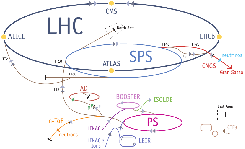
\includegraphics[width=.8\linewidth]{lhc_inj_chain}
    \caption{The LHC injection chain~\cite{LHCFAQ}.}
    \label{fig:lhc_inj_chain}
\end{figure}
%%% Local Variables:
%%% mode: latex
%%% TeX-master: "../search_for_DM_LED_with_ATLAS"
%%% End:


\section{The ATLAS Detector}
\label{sec:atlas-detector}

The ATLAS detector $\dots$
%%% Local Variables:
%%% mode: latex
%%% TeX-master: "../search_for_DM_LED_with_ATLAS"
%%% End:


\subsection{The Coordinate System}
\label{sec:coordinate-system}

The ATLAS detector uses a right handed coordinate system with the origin at the
nominal interaction point with the $z$-axis along the beam direction and the
$xy$ plane orthogonal to it. The positive $x$-axis goes from the interaction
point to the center of the LHC ring and the positive $y$-axis is defined as
pointing upwards. The A-side of the detector is defined as that with a positive
$z$-axis while the C-side has the negative $z$-axis.

The LHC beam are unpolarized and thus invariant under rotations around the beam
line axis, a cylindrical coordinate system is particularly convenient to
describe the detector geometry where:
\begin{equation}
  \label{eq:57}
  r = \sqrt{x^2 + y^2}, \quad \phi = \arctan \frac{y}{x}.
\end{equation}
A momentum dependent coordinate, the \emph{rapidity}, is commonly used in
particle physics for its invariance under Lorentz transformations. The rapidity
is defined as:
\begin{equation}
  \label{eq:58}
  y = \frac{1}{2} \ln \frac{E + p_z}{E - p_z}
\end{equation}
where $E$ is the energy of the particle and $p_z$ its momentum along the
$z$-axis. Rapidity intervals are Lorentz invariant. In the relativistic limit or
when the mass of the particle is negligible, the rapidity only depends on the
production angle of the particle with respect to the beam axis,
\begin{equation}
  \label{eq:59}
  \theta = \arctan \frac{\sqrt{p_x^2 + p_y^2}}{p_z}.
\end{equation}
This approximation is called \gls{eta} and is defined as:
\begin{equation}
  \label{eq:60}
  y \xrightarrow{p \gg m} \eta = - \ln \left( \tan \frac{\theta}{2} \right).
\end{equation}
A value of $\theta = 90^{\circ}$, perpendicular to the beam axis, corresponds to
$\eta = 0$. The spatial separation between particles in the detector is commonly
given in terms of a Lorentz invariant variable defined as:
\begin{equation}
  \label{eq:61}
  \Delta R = \sqrt{\Delta \phi^2 + \Delta \eta^2}.
\end{equation}

Other quantities used to describe the kinematics of the $pp$ interaction are the
\gls{pt} and the \gls{et} defined as $\pt = p \sin \theta$ and
$\et = E \sin \theta$ respectively.
%%% Local Variables:
%%% mode: latex
%%% TeX-master: "../search_for_DM_LED_with_ATLAS"
%%% End:


\subsection{The Inner Detector}
\label{sec:inner-detector}

The inner detector (ID) is designed to provide good track reconstruction,
precise momentum resolution and both primary and secondary vertex measurements
above a nominal $\pt$ threshold of 0.5~GeV and within the pseudorapidity
$|\eta| < 2.5$. It also provides electron identification over $|\eta| < 2.0$ for
energies between 0.5~GeV and 150~GeV\cite{ATLASPaper}. The ID is 6.2~m long and
has a radius of about 1.1~m, it is surrounded by a solenoidal magnetic field of
2~T. Its layout is schematized in Figure~\ref{fig:id} and, as can be seen, it is
composed of three sub-detectors. At the inner radius the \emph{pixel detector}
mostly determines the position of primary and secondary vertex. The silicon
sensors are 250~$\mu$m thick detectors that operate with an initial bias voltage
of $\sim$150~V that will increase up to 600~V after 10 years of operation. In
the middle layer of the ID the \emph{semiconductor tracker} (SCT) is designed to
give eight precision measurements per track which contributes to the primary and
secondary vertex position and momentum measurements. The silicon sensors are 285
$\pm 15 \mu$m thick and initially operated with a bias voltage of $\sim$150
position
\begin{figure}[!h]
  \centering
    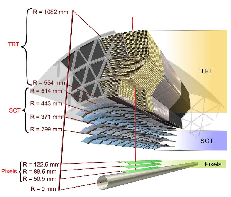
\includegraphics[width=.5\linewidth]{inner_detector}
    \caption{Schematic view of a charged track of 10~GeV $\pt$ that traverses
      the different ID sub-detectors. After traversing the beryllium pipe, the
      track passes through the three cylindrical silicon-pixel layers, the four
      layers of silicon-microstrip sensors (SCT) and the approximately 36 straws
      contained in the TRT within their support structure.}
    \label{fig:id}
\end{figure}
%%% Local Variables:
%%% mode: latex
%%% TeX-master: "../search_for_DM_LED_with_ATLAS"
%%% End:


\subsection{The Calorimeter}
\label{sec:calorimeters}

The main purpose of a calorimeter is to measure the energy of electrons, photons
and hadrons by mean of materials capable of completely absorb the energy of the
incoming particles transforming it in some measurable quantity. Calorimeters can
be classified in two categories, \gls{em} and \emph{hadronic} depending on the
particle they are designed to detect. The EM calorimeters are mainly used to
detect photons and electrons while the task of hadronic calorimeters is to
identify hadrons. Both types of calorimeters can be further divided into
\emph{sampling calorimeters} and \emph{homogeneous calorimeters}. Sampling
calorimeters alternates layers of a dense material used to absorb the energy of
incident particles (absorber) and an active material to collect the signal. The
interaction between the particles and the absorber produces a shower of
secondary particles with progressively degraded energy which is deposited in the
active material in form of charge or light that can be converted into
energy. Homogeneous calorimeters use only one material that serves both as an
absorber and an active material~\cite{Calorimetry}.

The ATLAS calorimeter is a sampling calorimeter covering up the $|\eta| < 4.9$
region the large $\eta$ coverage, ensures a good missing transverse momentum
measurement (see Section~\ref{sec:miss-transv-energy}); an illustration of the
system is shown in Figure~\ref{fig:calo}.

The EM calorimeter has a barrel and two end-caps, covering the $|\eta| < 1.475$
and $1.375 < |\eta| < 3.2$ region respectively. It uses \gls{lar} as active
material and lead as absorber in an accordion geometry that provides $\phi$
symmetry without azimuthal cracks. In the region $|\eta| < 1.8$ a presampler
consisting of a LAr active region is used to correct for electrons and photons
energy loss upstream of the calorimeter.

There are then three hadronic calorimeters: the \gls{tilecal}, the \gls{hec} and
the \gls{fcal}. The TileCal barrel and extended barrels cover the $|\eta| < 1.0$
and $0.8 < |\eta| < 1.7$ and uses steel as absorber and scintillating tiles
connected to photomultipliers tubes through wavelength shifting fibers for
readout as an active material. The HEC covers the $1.5 < |\eta| < 3.2$ region
and, to avoid drops in material density at the transition, it overlaps slightly
with the FCal that covers the $3.1 < |\eta| < 4.9$.

\begin{figure}[!h]
  \centering
    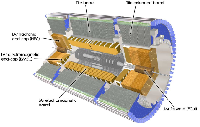
\includegraphics[width=.5\linewidth]{calorimeters}
    \caption{Cut-away view of the ATLAS calorimeter system.}
    \label{fig:calo}
\end{figure}
%%% Local Variables:
%%% mode: latex
%%% TeX-master: "../search_for_DM_LED_with_ATLAS"
%%% End:


\subsection{The Muon Spectrometer}
\label{sec:muon-spectrometer}

The Muon Spectrometer (MS) is designed to identify muons and measure their
momentum. It is divided in four sub-detectors, the Monitored Drift Tubes (MDT),
the Cathode Strip Chambers (CSC), the Resistive Plate Chambers (RPC), and the
Thin Gap Chamber (TGC) that. The sub-detectors are immersed in a magnetic field
generated by three different toroidal magnets, a barrel toroid covering the
$|\eta| < 1.4$ region and two end-caps magnets at $1.6 < |\eta| < 2.7$, which
produces a field almost perpendicular to the muon tracks.

The MDT covers the $|\eta| < 2.7$ region and provides a precise measurement of
the track coordinates in the principal bending direction of the magnetic
field. It uses drift tubes filled with an Ar (93\%) and CO$_2$ (3\%) gas mixture
and a tungsten-rhenium wire at 3080~V potential as anode. To reconstruct the
muon trajectory, the drift time of the ionized charges is used to determine the
minimum distance between the wire and the muon. The CSC covers the $2.0 < |\eta|
< 2.7$ region and is a multi-wire proportional chamber with cathodes segmented in
strips, one perpendicular to the anode wire, providing the precision coordinate,
and the other parallel to it (giving the transverse coordinate).


The RPC and the TGC cover the $|\eta| < 1.05$ and $1.05 < |\eta| < 2.7$ regions
respectively. They contribute to the Level 1 trigger providing bunch-crossing
identification, it allows to select high and low $\pt$ tracksand measure the
muon coordinate in the direction orthogonal to that determined by MDT and CSC.

\begin{figure}[!h]
  \centering
    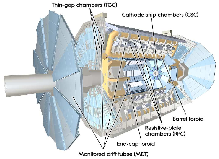
\includegraphics[width=.5\linewidth]{muon_spectro}
    \caption{Cut-away view of the ATLAS muon spectrometer.}
    \label{fig:muon_spectro}
\end{figure}
%%% Local Variables:
%%% mode: latex
%%% TeX-master: "../search_for_DM_LED_with_ATLAS"
%%% End:


\subsection{The Forward Detectors}
\label{sec:forward-detectors}

The ATLAS forward region is covered by three smaller detectors: the \gls{lucid},
the \gls{alfa} and the \gls{zdc}. LUCID~\cite{ForwardDetectors} is located at
$\pm 17$~m from the IP, it is designed to monitor the relative luminosity by
detecting the inelastic $pp$ scattering. The ZDC~\cite{ForwardDetectors} is
located at $\pm 140$~m from the IP, it consists of alternating layers of quartz
rods and tungsten plates designed to measure neutron at $|\eta| < 8.2$, its
purpose is to measure the centrality in heavy-ion
collisions. ALFA~\cite{ForwardDetectors} is located at $\pm 240$~m from the IP
and is designed to measure the absolute luminosity via elastic scattering at
small angles.
%%% Local Variables:
%%% mode: latex
%%% TeX-master: "../search_for_DM_LED_with_ATLAS"
%%% End:


\subsection{Track reconstruction}
\label{sec:track-reconstruction}

Object reconstruction is the process that associates the signal left in the
detector by charged particles to physical objects through a series of
algorithms.

Charged particles that move through a homogeneous solenoidal magnetic field
along the $z$ direction, follow helical trajectories. The projection of a helix
on the $xy$ plane is a circle and, in order to uniquely parametrize a helix in
three dimensions, five parameters are needed. A common choice is to use the
\emph{perigee} parameters, where the perigee is the point of closest approach to
the beam axis. With this choice, the five parameters are:
\begin{itemize}
\item The signed curvature $C$ of the helix, defined as $C = q / 2R$ where $q$ is
  the particle charge and $R$ is the radius of the helix. This is related to the
  transverse momentum $\pt = qB / C$, where $B$ is the magnetic field measured
  in Tesla, C is measured in m$^{-1}$ and $\pt$ in GeV / c$^2$.
\item The distance of closest approach $d_0$ in the $xy$ plane.
\item The $z$ coordinate of the point of closest approach, denoted by $z_0$.
\item The azimuthal angle $\phi_0$ of the tangent to this point.
\item The polar angle $\theta$ to the $z$-axis.
\end{itemize}
The perigee and the track parameters are schematized in Figure~\ref{fig:track_par}

\mbox{}

\textbf{try to find what \emph{LooseTrackOnly} is that I mention
  on~\autoref{sec:electrons}}
\begin{figure}[!h]
  \centering
    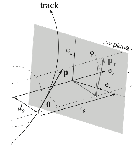
\includegraphics[width=.5\linewidth]{track_parameters}
    \caption{Perigee parameters}
    \label{fig:track_par}
\end{figure}
%%% Local Variables:
%%% mode: latex
%%% TeX-master: "../search_for_DM_LED_with_ATLAS"
%%% End:


\subsection{The Trigger System}
\label{sec:trigger-system}

The bunch crossing rate at LHC is 40~MHz for a bunch spacing of 25~ns (about 7
meters). Each event recorded by ATLAS requires $\approx 1.4$~MB of disk space,
with approximately 20 to 50 collisions per bunch crossing, the storage space
required to record all the events in a second would be $\approx 60$~TB. This is
not feasible thus only the most interesting events are selected and stored on
disk. The \emph{trigger system} decides whether to keep or not a collision event
for later studies, it consists of a hardware based \gls{l1} trigger and a
software based \gls{hlt}.

The L1 trigger determines \gls{rois} in the detector using custom hardware and
coarse information from the calorimeter and the muon system. The L1 trigger is
capable of reducing the event rate to 100~kHz with a decision time for a L1
accept of 2.5~$\mu$s. The RoIs from the L1 trigger are sent to the HLT where
different algorithms are run using the full detector information and reducing
the L1 output rate to 1~kHz with a processing time of about
200~ms~\cite{trigger}. A schematic overview of the ATLAS trigger and data
acquisition system is shown in Figure~\ref{fig:trigger_system}.

In the monojet analysis presented in this thesis, the HLT\_xe70 trigger is used,
it receives an L1 accept that selects events with a missing energy (see
Section~\ref{sec:miss-transv-energy}) greater than 50~GeV, no muons are used in
the reconstruction of the missing energy at the trigger level. The events that
survive L1 are then passed to the HLT level, where events with a missing energy
greater than 70~GeV are selected.
% \begin{figure}[!h]
%   \centering
%     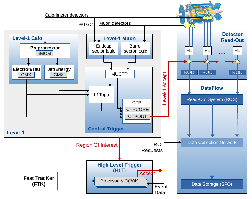
\includegraphics[width=.7\linewidth]{trigger_system}
%     \caption{Schematic view of the ATLAS trigger and data acquisition system.}
%     \label{fig:trigger_system}
% \end{figure}
%%% Local Variables:
%%% mode: latex
%%% TeX-master: "../search_for_DM_LED_with_ATLAS"
%%% End:


\chapter{Noise Studies with the Tile Calorimeter}
\label{cha:noise-studies-with}

\section{Calorimetry}
\label{sec:calorimetry}

The particle interactions with matter cause them to lose energy. The particle's
energy and its type determines the processes causing the energy loss; these can
be of two kind, \emph{electromagnetic} and \emph{hadronic}. In this section a
brief overview of the physics behind the two is given.
%%% Local Variables:
%%% mode: latex
%%% TeX-master: "../search_for_DM_LED_with_ATLAS"
%%% End:


\subsection{The Electromagnetic Shower}
\label{sec:electr-show}

High energy electrons and photons can lose energy by \emph{ionization} or
\emph{radiation}. When electrons with energies greater than $\sim 10$~MeV
interacts with the electromagnetic field generated by the absorber layer nuclei,
a deceleration and thus a loss of energy in form of a photon
(\emph{Bremsstrahlung}) is experienced. Photons in this energy range produce
mostly electron-positron pairs.

Electrons and photons with a sufficient amount of energy interacting with an
absorber, produce secondary photons through Bremsstrahlung or secondary
electrons and positrons by pair production. These secondary particles will
produce more particles through the same mechanisms giving rise to a shower of
particles with progressively lower energies. At this stage, electrons lose their
energy through ionization and thermal excitation of the active material atoms
while photons lose energy through the Compton scattering and the photoelectric
effect. This process goes on until the energy of the electrons falls below a
critical energy, $\epsilon$, where ionization and excitation becomes the
dominant effects~\cite{Calorimetry}.
%%% Local Variables:
%%% mode: latex
%%% TeX-master: "../search_for_DM_LED_with_ATLAS"
%%% End:


\subsection{Hadronic Shower}
\label{sec:hadronic-shower}

In a similar way to the electromagnetic shower, hadrons lose energy through
strong interaction with the calorimeter material. The strong interaction is
responsible for the production of energetic secondary hadrons with momenta
typically at the GeV scale and nuclear reactions such as excitation or nucleon
spallation in which neutrons and protons are released from the nuclei with a
characteristic energy at the MeV scale.

The hadron produced are mainly pions, of these, 90\% are neutral pions which
decay to photons ($\pi \rightarrow \gamma \gamma$). The photons produced this
way will initiate an electromagnetic shower as described in
Section~\ref{sec:electr-show} transferring energy from the hadronic part to the
electromagnetic and not contributing any more to hadronic processes. The
nucleons released by excitation or nuclear spallation, require an energy equal
to their binding energy to be released and are not recorded as a contribution to
the calorimeter signal thus producing a form of \emph{invisible energy}. Some
detectors can compensate for the loss of invisible energy, these are called
\emph{compensated calorimeters}~\cite{Calorimetry}.
%%% Local Variables:
%%% mode: latex
%%% TeX-master: "../search_for_DM_LED_with_ATLAS"
%%% End:


\subsection{Energy Resolution}
\label{sec:energy-resolution}

The energy resolution of a detector measure its capability of distinguishing
between radiation of similar energies; the better the energy resolution, the
better it can separate energy peaks belonging to different decays.

The energy resolution, in general, can be written as:
\begin{equation}
  \label{eq:64}
  \frac{\sigma_E}{E} = \frac{a}{\sqrt{E}} \oplus \frac{b}{E} \oplus c,
\end{equation}
where the $\oplus$ symbol indicates a quadratic sum. The first term in the
equation is the \emph{stocastic term}, it is due to fluctuations related to the
physical development of the shower. In homogeneous calorimeters, this term is
small because the energy deposited in the active volume by a monochromatic beam
of particles is constant for each event. In a sampling calorimeter, the active
layers are interleaved with absorber layers thus the energy deposited in the
active material fluctuates event by event. These are called \emph{sampling
  fluctuations} and represent the greatest limitation to energy resolution in
these kind of calorimeters due to the variation in the number of charged
particles which cross the active layers. The second term in eq.~\eqref{eq:64} is
called the \emph{noise term}, it comes from the electronic noise of the detector
readout chain. Sampling or homogeneous calorimeters which collect the signal in
the form of light, using for example a photo-multiplier tube with a high gain
multiplication of the signal with a low electronic noise, can achieve low levels
of noise. Calorimeters that collect the signal in form of charge, must use an
pre-amplifier having thus a higher level of noise. In sampling calorimeters, the
noise term can be further reduced by increasing the sampling fraction, this way
there is a larger signal coming from the active material and a higher
noise-to-signal ratio. The last term of the equation is the \emph{constant
  term}, it does not depend on the energy of the particles but includes all the
non uniformities in the detector response such as instrumental effect, radiation
damage, detector aging or the detector geometry~\cite{Calorimetry}.
%%% Local Variables:
%%% mode: latex
%%% TeX-master: "../search_for_DM_LED_with_ATLAS"
%%% End:


\section{The ATLAS TileCal}
\label{sec:atlas-tilecal}

TileCal is the central hadronic calorimeter of the ATLAS experiment covering the
$|\eta| < 1.7$ region. It is designed for energy measurement of hadrons, jets,
tau particles and also contributes to the measurement of missing transverse
energy (see Section~\ref{sec:miss-transv-energy}). TileCal is a scintillator
steel non compensating sampling calorimeter, the scintillation light produced in
the tiles is transmitted by wavelength shifting fibers to \glspl{pmt}. The
analog signals from the PMTs are amplified, shaped and digitized by sampling the
signal every 25~ns. The TileCal front end electronics read out the signals
produced by about 10000 channels measuring energies ranging from 30~MeV to
2~TeV. The readout system is responsible for reconstructing the data in real
time. The digitized signals are reconstructed with the Optimal Filtering
algorithm (see Section~\ref{sec:optimal-filtering}), which computes for each
channel the signal amplitude, time and quality factor at the required high rate.

TileCal is designed as one \gls{lb} and two \gls{eb}. The barrels are further
divided, according to their geometrical position on the $z$-axis, in partitions
called EBA, LBA, EBC and LBC (see Section~\ref{sec:coordinate-system}). Each
partition consists of 64 independent wedges (see Figure~\ref{fig:tile_mod})
along the azimuthal direction called \emph{modules}; the LBA and EBA partitions
are shown in Figure~\ref{fig:tile_cells}.

\begin{figure}[!h]
  \centering
    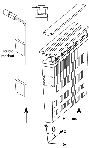
\includegraphics[width=.5\linewidth]{tile_module}
    \caption{Cut away showing the optical read out and design of a TileCal
      module.}
    \label{fig:tile_mod}
\end{figure}

Between the LB and the EB there is a 600~mm gap needed for the ID and the LAr
cables, electronics and services. Part of the gap contains the \gls{itc}, a
detector designed to maximize the active material while leaving enough space for
services and cables. The ITC is an extension of the EB and it occupies the 0.8 <
$|\eta|$ < 1.6 region. The combined 0.8 < $|\eta|$ < 1.0 part is called
\emph{plug} and in the 1.0 < $|\eta|$ < 1.6 region, due to the very limited
space, the ITC is composed of only scintillator. The scintillators between 1.0 <
$|\eta|$ < 1.2 are called \emph{gap scintillators}, while those between 1.2 <
$|\eta|$ < 1.6 are called \emph{crack scintillators}. The plug and the gap
scintillators mainly provide hadronic shower sampling while the crack
scintillator, which extends to the region between the barrel and the end-cap
cryostats, samples the electromagnetic shower in a region where the normal
sampling is impossible due to the dead material of the cryostat walls and the ID
cables.

TileCal is also divided in longitudinal layers, the A, BC and D layers as shown
in Figure~\ref{fig:tile_cells}. The two innermost layers have a
$\Delta \eta \times \Delta \phi$ segmentation of $0.1 \times 0.1$ while in the
outermost, the segmentation is $0.1 \times 0.2$. Each layer is logically divided
into \emph{cells} by grouping together in the same PMT the fibers coming from
different scintillator tiles belonging to the same radial depth. The gap/crack
scintillators are also called E layer cells.

The energy resolution for jets of ATLAS is:
\begin{equation}
  \label{eq:65}
  \frac{\sigma_E}{E} = \frac{50\%}{\sqrt{E}} \oplus 3\%
\end{equation}
for $|\eta| < 3$. The 3\% constant term becomes dominant for high energy hadrons
where an increase in energy resolution is expected~\cite{TileCal}.

\begin{figure}[!h]
  \centering
    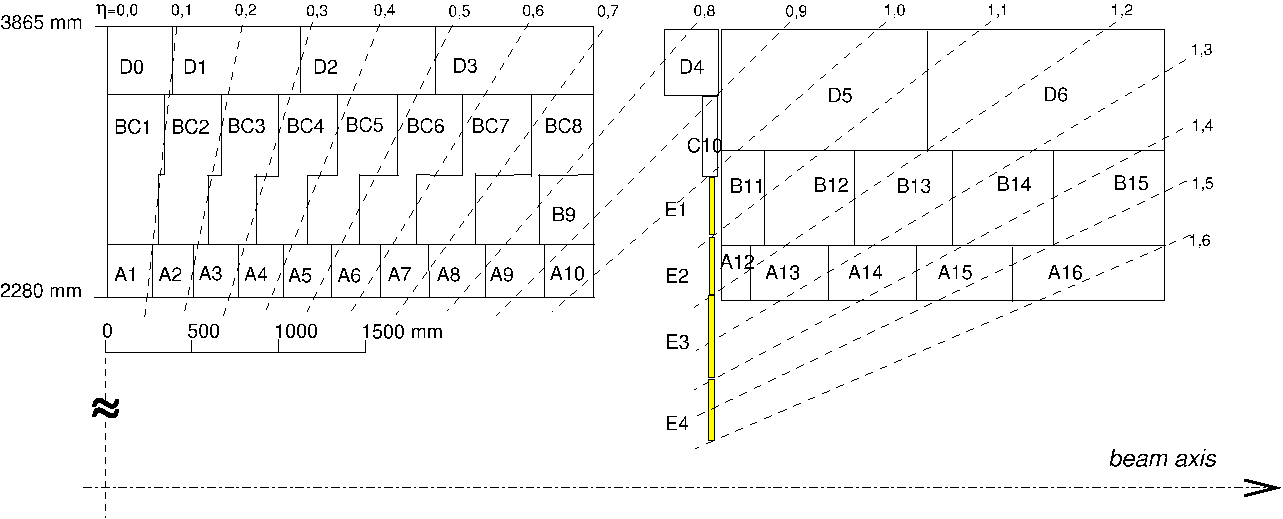
\includegraphics[width=\linewidth]{tile_cells}
    \caption{Schematic view of the TileCal scintillator structure~\cite{TileCalPub}.}
    \label{fig:tile_cells}
\end{figure}
%%% Local Variables:
%%% mode: latex
%%% TeX-master: "../search_for_DM_LED_with_ATLAS"
%%% End:


\subsection{Signal Reconstruction}
\label{sec:sign-reconstr}

The TileCal cells are read out by two PMTs with the exception of the E layer
cells that are connected to only one photomultiplier tube using \gls{wsf}. Each
PMT is associated to an electronic read-out channel. The current pulse from the
PMTs is shaped and amplified by the 3-in-1 card. There are two possible gains:
\gls{hg} and \gls{lg}, with an amplification ratio of 64. The 3-in-1 card forms
the front-end electronics of the read-out chain and provides three basic
functions: shaping of the pulse, charge injection calibration and slow
integration of the PMT signals for monitoring and calibration~\cite{TileCal}
(\textbf{don't really know much about this}). Up to twelve 3-in-1 cards are
serviced by a motherboard that provides power and individual control signals.
The amplified signal is sent to two \glspl{adc} synchronous with the 40~MHz LHC
clock thus sampling the signal every 25~ns. For optimization and efficiency
reasons, 7 samples for each pulse are taken and sent to the \glspl{rod} for a L1
accept.
%%% Local Variables:
%%% mode: latex
%%% TeX-master: "../search_for_DM_LED_with_ATLAS"
%%% End:


\subsubsection{Optimal Filtering}
\label{sec:optimal-filtering}

The seven samples are used to reconstruct the amplitude of the pulse using the
\gls{of} method. The estimate of the amplitude is given by:
\begin{equation}
  \label{eq:66}
  \hat{A} = \sum_{i = 0}^7 a_i S_i
\end{equation}
where $S_i$ are the digitized samples expressed in ADC counts and $a_i$ are
computed weights that minimize the effect of the electronic noise on the
amplitude reconstruction. The procedure minimizes the variance of the amplitude
distribution. In order to make the amplitude reconstruction independent from
phase and signal baseline due to electronic noise (\emph{pedestal}), the
following constraints are used:
\begin{equation}
  \label{eq:67}
  \sum_{i = 0}^7 g_i a_i = 0
\end{equation}
\begin{equation}
  \label{eq:68}
  \sum_{i = 0}^7 g'_i a_i = 0
\end{equation}
\begin{equation}
  \label{eq:69}
  \sum_{i = 0}^7 a_i = 0
\end{equation}
where $g_i$ and $g'_i$ are the pulse shape function from the shaper and its
derivative~\cite{OptimalFilter}.
%%% Local Variables:
%%% mode: latex
%%% TeX-master: "../search_for_DM_LED_with_ATLAS"
%%% End:


\subsubsection{The TileCal Calibration}
\label{sec:tilecal-calibration}

\begin{figure}[!h]
  \centering
    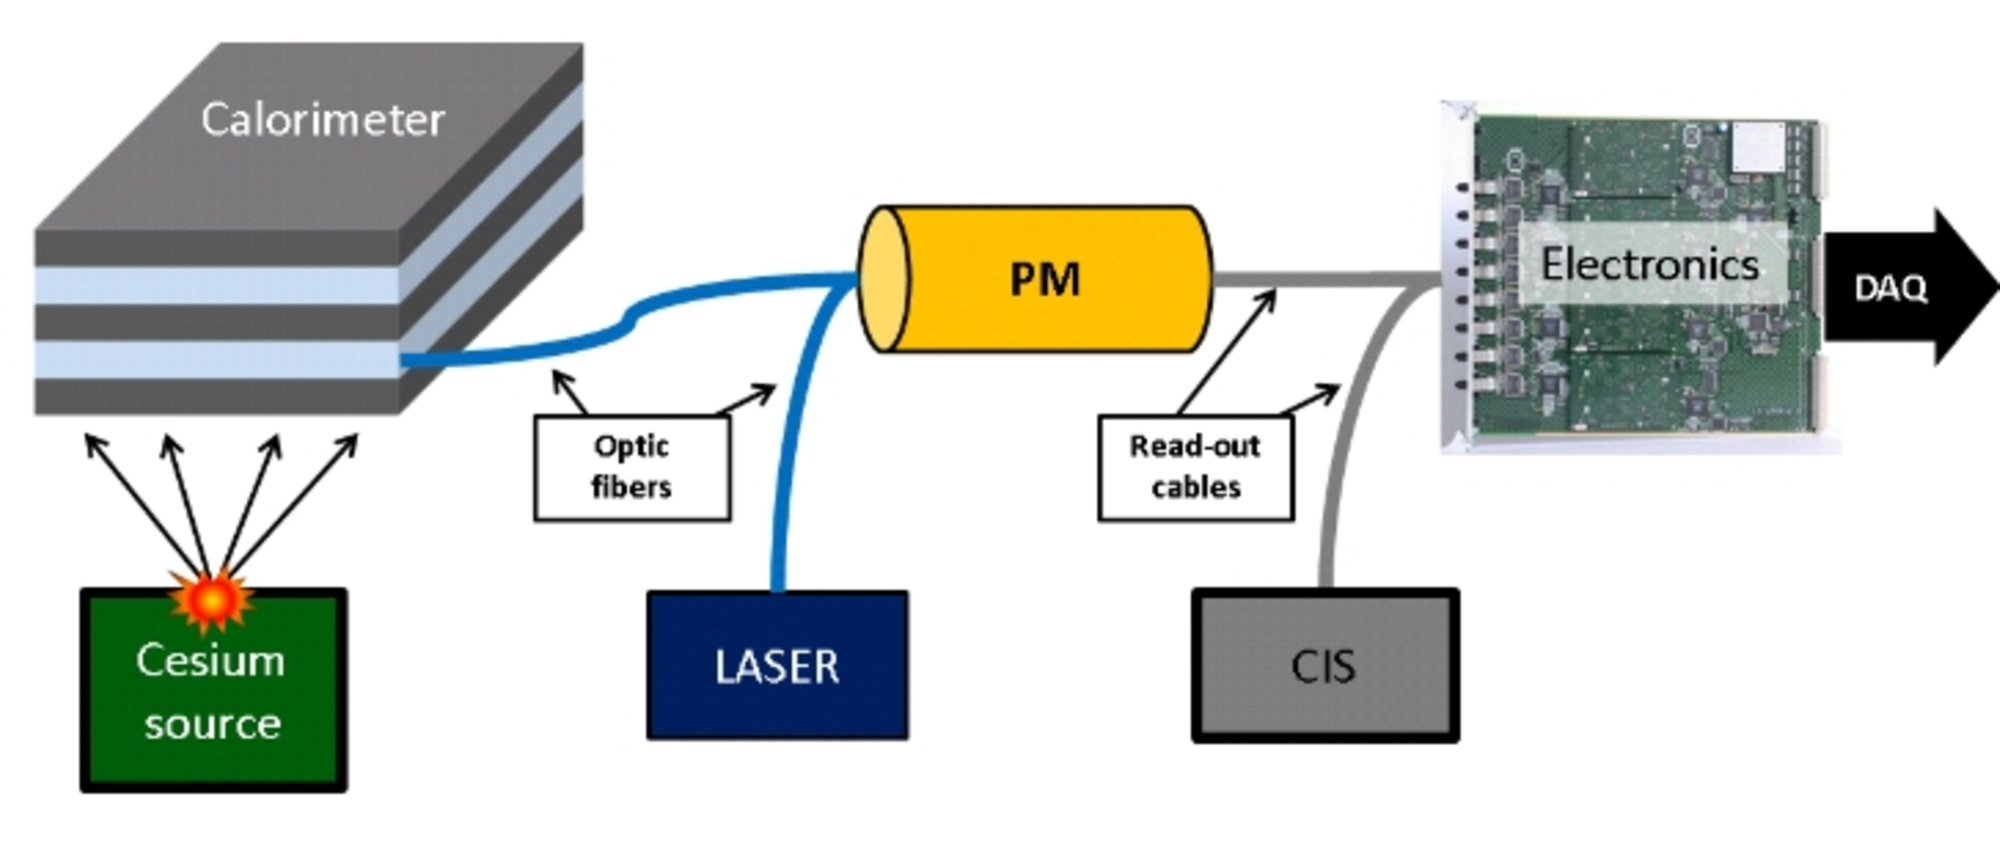
\includegraphics[width=.5\linewidth]{calibration_chain}
    \caption{The ATLAS TileCal calibration chain.}
    \label{fig:cali_chain}
\end{figure}

The energy deposited in the calorimeter cell is proportional to the
reconstructed amplitude. The amplitude is originally measured in ADC counts and
needs to be converted in GeV for physics analysis using the formula:
\begin{equation}
  \label{eq:70}
  E[GeV] = \hat{A}[ADC] \times C_{ADC \rightarrow pC} \times C_{\text{laser}}
  \times C_{Cs} \times C_{pC \rightarrow GeV}
\end{equation}
where $\hat{A}[ADC]$ is the amplitude estimate in ADC counts, $C_{ADC \rightarrow
pC}$ is determined using the \gls{cis}, $C_{pC \rightarrow
  GeV}$ is measured during testbeam using electrons with a well defined energy
and converts the deposited charge to energy in GeV, the laser system allows to
determine the value of the $C_{\text{laser}}$ constant while the Cesium sets the
$C_{Cs}$ factor.

The CIS calibrates the read out electronics by injecting a known charge and
measuring the resulting response of the electronics. The \emph{laser} system
main purpose is to monitor the photomultipliers tubes and the downstream
electronics. Well calibrated light pulses are sent to the PMTs and by
reconstructing the signal it is possible to extract the PMTs' gain. The
\emph{cesium} system, circulate a Cs source through each scintillating tile
using an hydraulic system, the PMTs signal is continuously read out through an
integrator. This system allows to adjust the EM scale and equalize the
calorimeter cell response.
%%% Local Variables:
%%% mode: latex
%%% TeX-master: "../search_for_DM_LED_with_ATLAS"
%%% End:


\subsection{Electronic Noise}
\label{sec:electronic-noise}

TileCal periodically performs sets of recorded event (\emph{runs}) with no
signal in the PMTs, called \emph{pedestal runs}; during these runs, each channel
is read out using both, HG and LG for about 100000 events. These events are
sampled every 25~ns in 7 samples as in normal physic runs and are normally
distributes around a mean value called \emph{pedestal}. The \gls{rms} of the
pedestal is defined as \emph{noise}. Pedestal runs are used to calculate
different parameters that allow to describe the electronic noise called
\emph{noise constants}. Two different sets of noise constants are computed:
\emph{Digital Noise} (or \emph{Sample Noise}) and \emph{Cell Noise}.
%%% Local Variables:
%%% mode: latex
%%% TeX-master: "../search_for_DM_LED_with_ATLAS"
%%% End:


\subsubsection{Digital Noise}
\label{sec:digital-noise}

The digital noise is measured in ADC counts for each PMT in both gains, HG and
LG\@. The noise constants stored are the RMS of the seven samples within each
event, also called \gls{hfn} and the RMS of the first digitized sample in each
event or \gls{lfn}. The digital noise is used for monitoring and for \gls{mc}
noise simulation.
%%% Local Variables:
%%% mode: latex
%%% TeX-master: "../search_for_DM_LED_with_ATLAS"
%%% End:


\subsubsection{Cell Noise}
\label{sec:cell-noise}

Excluding the E layer cells that are connected only to one PMT, the cell noise
is the combination of the two readout channels of a cell where the digital noise
from the PMTs is added quadratically and converted in MeV using the calibration
constants and eq.~\eqref{eq:70}. This combination results in four possible gain
combinations: \gls{hghg}, \gls{lglg}, \gls{lghg} and \gls{hglg}. The cell noise
is used to identify the seed cells in the topocluster algorithm (see
Section~\ref{sec:topocluster}).

Figure~\ref{fig:non_gaussianity} shows a comparison between the cell noise and
the fitted $\sigma$ parameter of a normal distribution. The ratio RMS / $\sigma$
= 1 indicates a perfect agreement between the measured and the fitted amplitude
distribution for a single Gaussian hypothesis. The blue square in the plot
indicate the comparison for an old model of \glspl{lvps} while the red square
refers to the currently used LVPSs. It can be seen that with the old model of
\glspl{lvps} the ratio RMS / $\sigma$ can be large indicating a non Gaussian
behavior of the electronic noise. For this reason a double Gaussian distribution
is used to fit the energy distribution with the probability density function
defined as:
\begin{equation}
  \label{eq:71}
  f_{2g} = \frac{1}{1 + R} \left( \frac{1}{\sqrt{2 \pi} \sigma_1} e^{-
      \frac{x^2}{2 \sigma_1^2}} + \frac{R}{\sqrt{2 \pi} \sigma_2} e^{-
      \frac{x^2}{2 \sigma_2^2}} \right)
\end{equation}
where $R$ is the relative normalization of the two Gaussians and
$\sigma_1, \sigma_2$ and $R$ are independent parameters. These three are used to
define the region $\sigma_{\text{eff}}(E)$ where the significance for the double
Gaussian is the same as the one $\sigma$ region for a single Gaussian,
i.e.
$\int_{- \sigma_{\text{eff}}}^{\sigma_{\text{eff}}} f_{2g} =
0.68$~\cite{TileReadiness}.
In terms of $\sigma_{\text{eff}}$, for an energy deposit $E$, the significance
can be expressed as:
\begin{equation}
  \label{eq:72}
  \frac{E}{\sigma_{\text{eff}}(E)} = \sqrt{2}\ \text{Erf}^{- 1} \left( \frac{\sigma_1
      \text{Erf} \left(\frac{E}{\sqrt{2 \sigma_1}} \right) + R \sigma_2 \text{Erf}
    \left( \frac{E}{\sqrt{2 \sigma_2}} \right)}{\sigma_1 + R \sigma_2} \right)
\end{equation}
where Erf is the error function. Equation~\ref{eq:72} is the input to the
calorimeter cell clustering algorithm discussed in more details in
\cref{sec:topocluster}, moreover this definition allows to use the same unit to
describe the noise for both the TileCal and LAr calorimeters. The region
$\sigma_{\text{eff}}(E)$ is commonly referred to as \emph{cell noise} and
together with the three double Gaussian parameters ($\sigma_1$, $\sigma_2$ and
R) is stored in the COOL database.

\begin{figure}[!h]
  \centering
    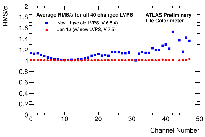
\includegraphics[width=.8\linewidth]{non_gaussianity}
    \caption{Comparison between the TileCal electronic noise, measured as the
      RMS of the reconstructed amplitude distribution in pedestal runs and the
      $\sigma$ of the Gaussian fit of the distribution for the old and new
      LVPS~\cite{TileCalNoisePub}.}
    \label{fig:non_gaussianity}
\end{figure}
%%% Local Variables:
%%% mode: latex
%%% TeX-master: "../search_for_DM_LED_with_ATLAS"
%%% End:


\section{The 2011 ATLAS Run I Reprocessing}
\label{sec:2011-atlas-run}

As new information about the detector becomes available, an update of the
calibration constants and thus of the reconstructed energy must be performed;
this procedure is called \emph{reprocessing}. In 2011 an update of the laser and
cesium calibration analysis procedure were performed together with an update of
which cells were considered good or bad. These updates required a recalculation
of the cell noise.
%%% Local Variables:
%%% mode: latex
%%% TeX-master: "../search_for_DM_LED_with_ATLAS"
%%% End:


\subsection{Perfromance}
\label{sec:perfromance}

Insert this part

\begin{figure}[!h]
  \centering
    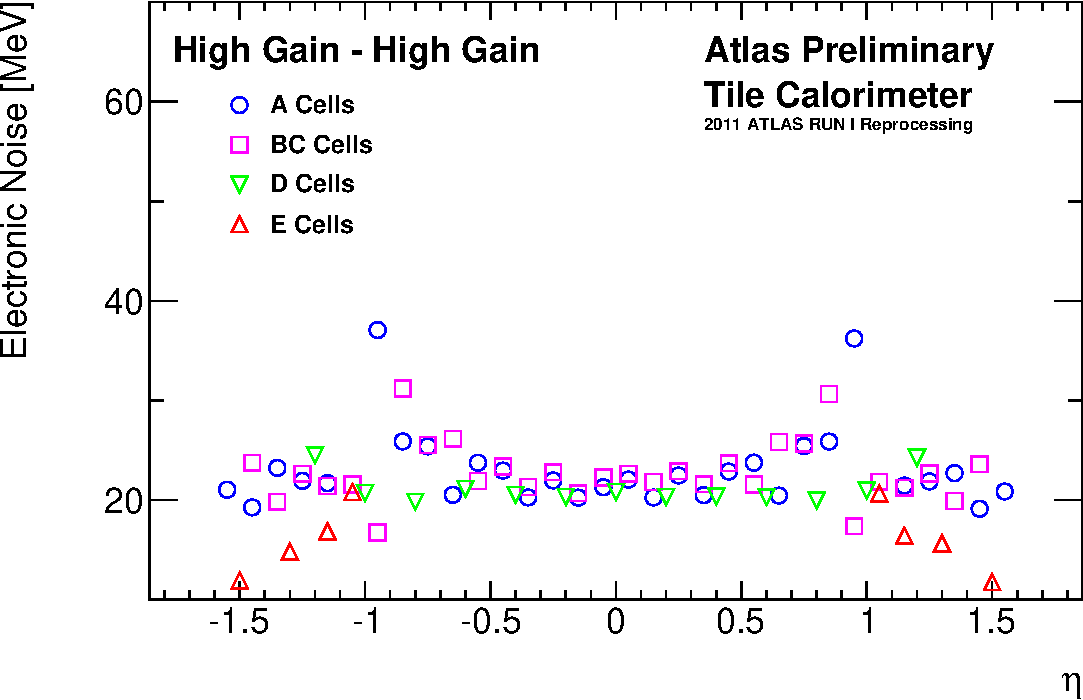
\includegraphics[width=.5\linewidth]{noise_avg_hghg}
    \caption{}
    \label{fig:noise_avg_hghg}
\end{figure}
%%% Local Variables:
%%% mode: latex
%%% TeX-master: "../search_for_DM_LED_with_ATLAS"
%%% End:


\subsection{Validity Checks}
\label{sec:validity-checks}

A certain set of calibration constants is valid over a period of time called
\gls{iov}. The cell noise can vary due to a change in the calibration, the
digital noise or the channel status in a particular run. This change must be
consistent and checked.

The different TileCal subsystems (laser, CIS, etc.) all use a common software
framework, \gls{tucs}, to perform validity checks on a number of different
studies. To test the stability over time of the updated noise constants, a set
of python scripts was developed to expand the TUCS functionality. These scripts
allow to visually display the relative change of the cell noise and digital
noise constants, the channel status and the ratio between the cell noise and a
variable called RMS$_\text{eff}$ and defined as:
\begin{equation}
  \label{eq:73}
  \text{RMS}_{\text{eff}} = \sqrt{(1 - R) \sigma_1^2 + R \sigma_2^2}
\end{equation}
where $\sigma_1$, $\sigma_2$ and R are the free parameter in the double Gaussian
model (see Section~\ref{sec:cell-noise}).  The ratio $\sigma$ /
RMS$_\text{eff}$, where $\sigma$ is the cell noise, can be used to test the
goodness of the double Gaussian model: if $\sigma$ / RMS$_\text{eff}$ equals
one, the double Gaussian well models the noise, if it is larger, it means that
there is noise that is not well described by it.

Figure~\ref{fig:jumps} shows the time evolution plot for two representative
TileCal cells. In Figure~\ref{fig:no_jumps} it can be seen that cell number 2 in
the BC layer (BC2) of the 41st module in the C side of LB (LBC 41) is stable
over several pedestal runs. In Figure~\ref{fig:with_jumps} on the other hand, it
is possible to see a variation in the cell noise and, accordingly, of the
$\sigma$ / RMS$_{\text{eff}}$ without a compatible variation in the calibration,
in the digital noise constants or in the channel status. The term \emph{jump}
will be used in the following to indicate a variation in the cell noise not
compatible with a change in the other quantities.

\begin{figure}[!h]
  \centering
  \begin{subfigure}[t]{.48\linewidth}
    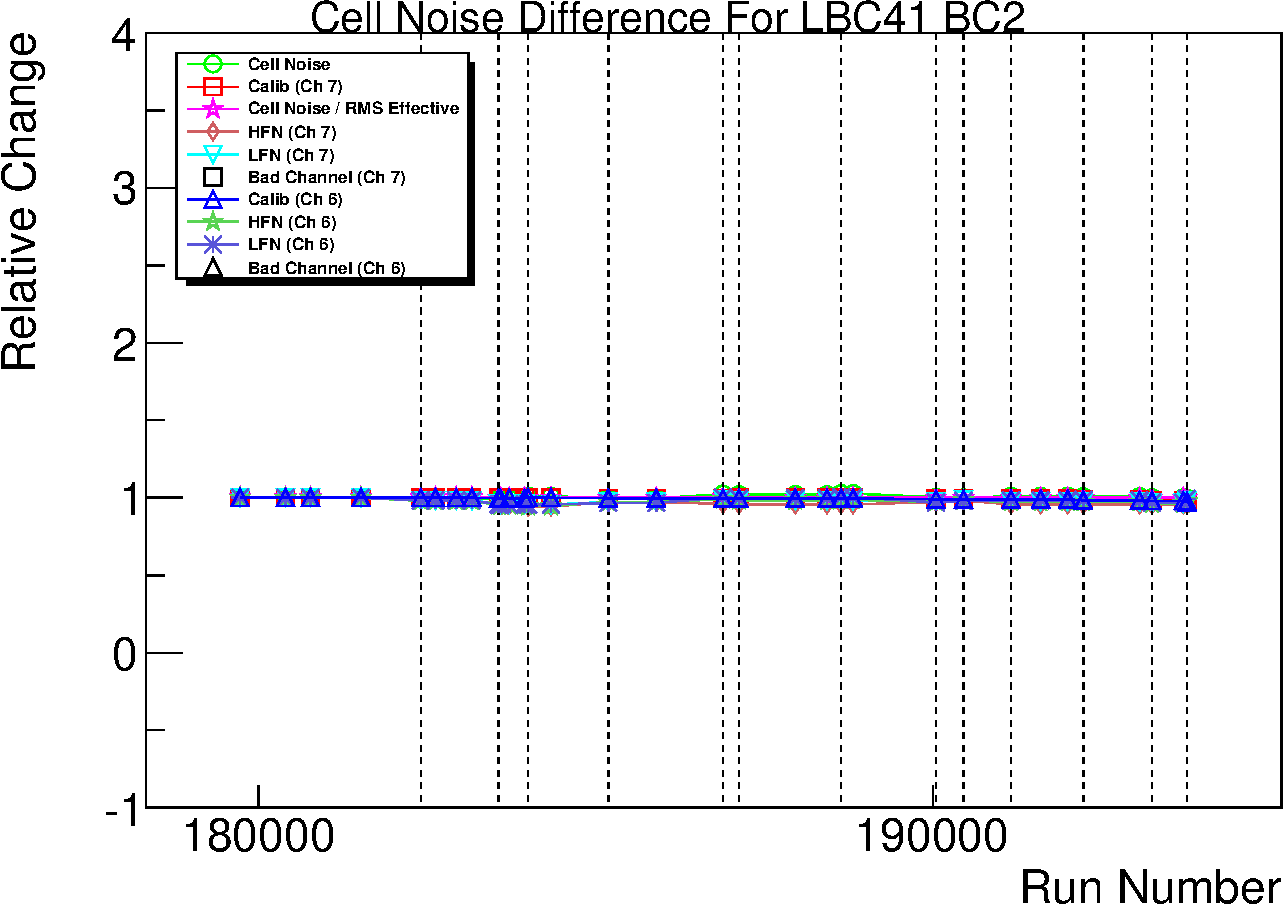
\includegraphics[width=\linewidth]{no_jumps}
    \caption{}
    \label{fig:no_jumps}
  \end{subfigure}
  \begin{subfigure}[t]{.48\linewidth}
    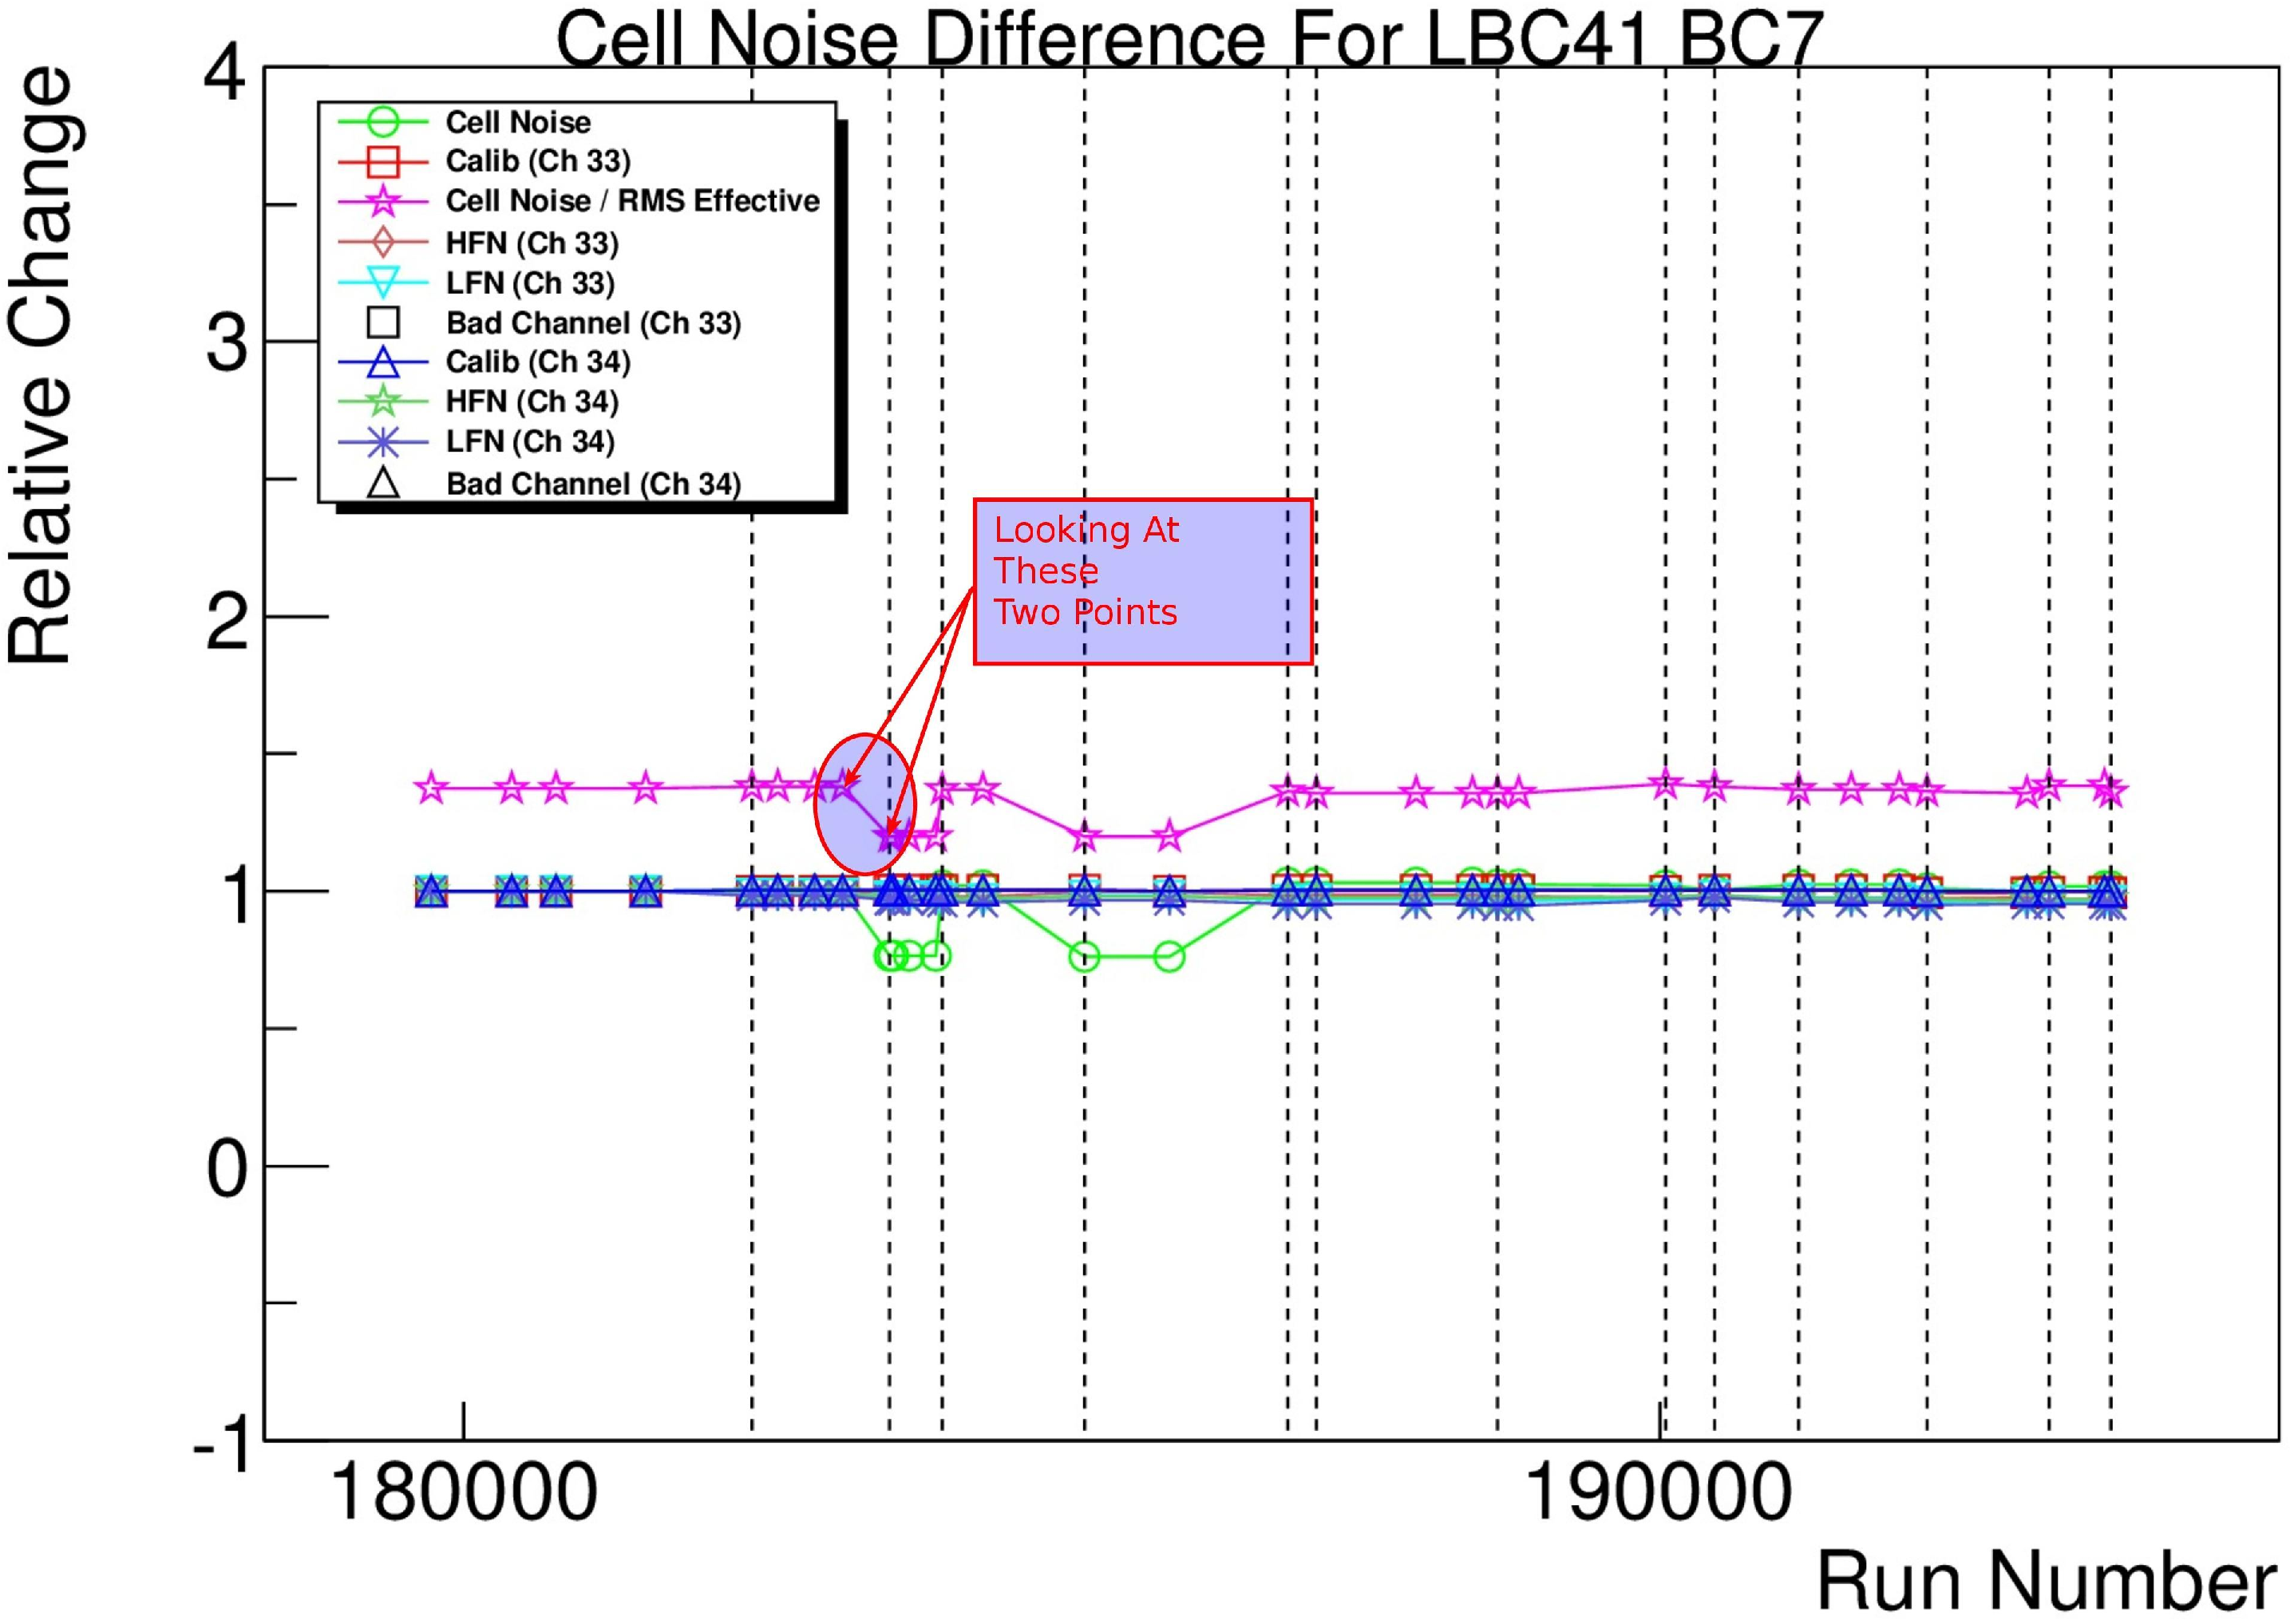
\includegraphics[width=\linewidth]{with_jumps}
    \caption{}
    \label{fig:with_jumps}
  \end{subfigure}
  \caption{Time evolution plots for two different representative cells in the
    calorimeter. The plot shows the change relative to the first run considered
    of several quantities for different IOVs (vertical dashed lines).}
  \label{fig:jumps}
\end{figure}

This problem was investigated by writing a software to manually fit the pulse
shape and calculate the noise constants focusing on two specific IOVs,
$[183110, 183382[$ and $[183382, 183515[$. Some calorimeter cells without jump
were used to validate the noise constants calculated with the fit and those
stored in the COOL database. Figure~\ref{fig:no_jump_fit} shows the control cell
energy distribution with the double Gaussian fit superimposed for two runs where
the jump was present in other cells. The results for the ratio of the amplitude
of the double Gaussian model (R), the RMS$_{\text{eff}}$ and the $\sigma$ /
RMS$_{\text{eff}}$ obtained with the fit are:
\begin{equation}
  \begin{cases}
    R : 0.0003 \\
    \text{RMS}_{\text{eff}}: 20.12 \\
    \sigma / \text{RMS}_{\text{eff}}: 0.998
  \end{cases}
  \to
  \begin{cases}
    R : 0.0002 \\
    \text{RMS}_{\text{eff}} : 20.07 \\
    \sigma / \text{RMS}_{\text{eff}}: 0.995.
  \end{cases}
  \label{eq:74}
\end{equation}
They are in good agreement with the values stored in the COOL database and
reported in Table~\ref{tab:no_jump_fit}.

\begin{figure}[!h]
  \centering
  \begin{subfigure}[t]{.48\linewidth}
    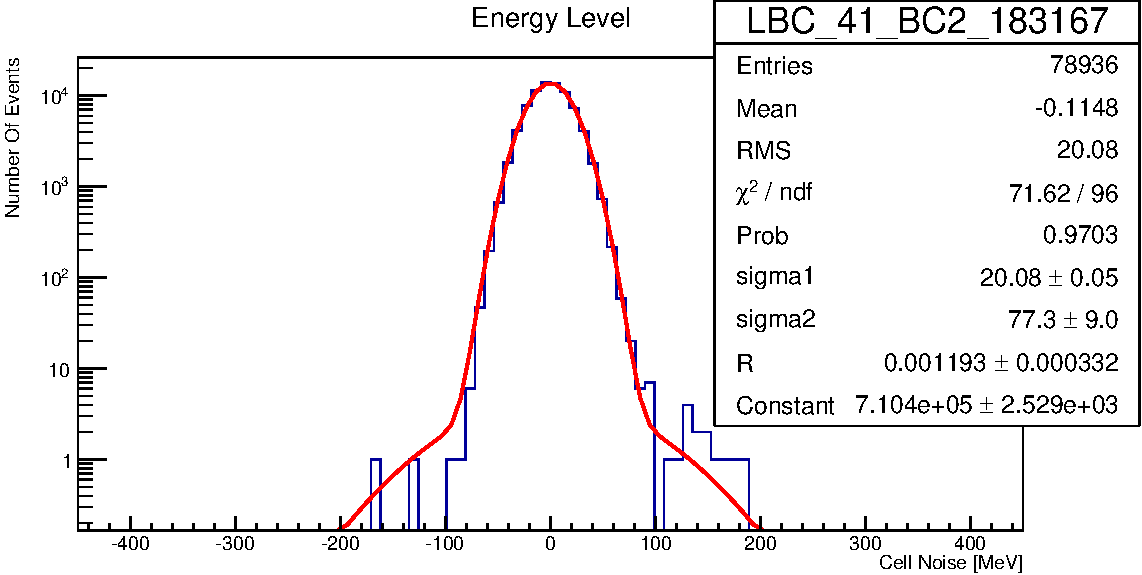
\includegraphics[width=\linewidth]{no_jump_fit_before}
    \caption{Fit before jump.}
    \label{fig:no_jump_fit_before}
  \end{subfigure}
  \begin{subfigure}[t]{.48\linewidth}
    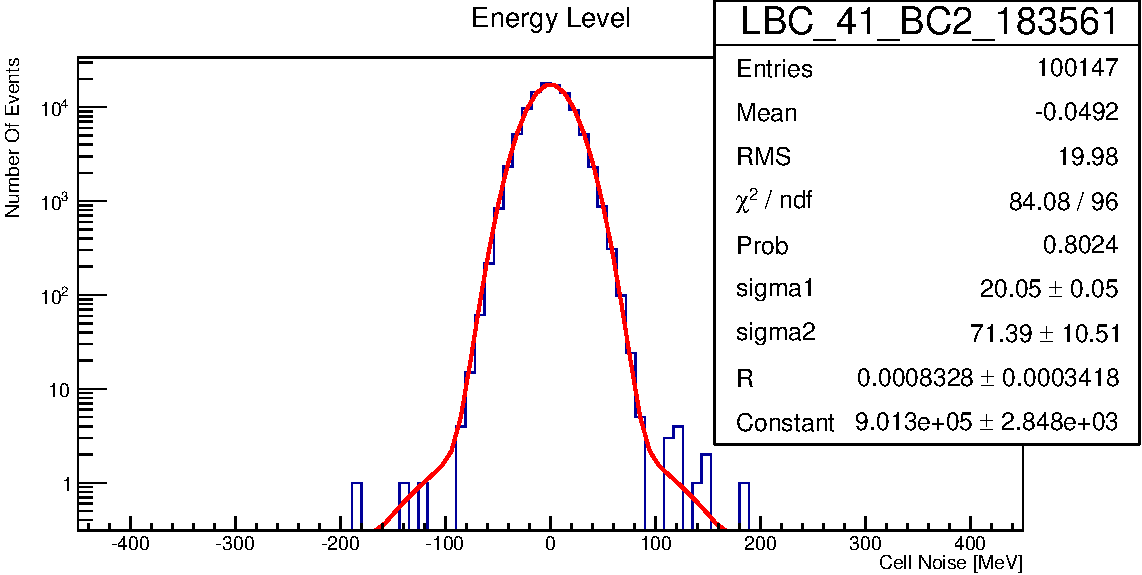
\includegraphics[width=\linewidth]{no_jump_fit_after}
    \caption{Fit after jump.}
    \label{fig:no_jump_fit_after}
  \end{subfigure}
  \caption{Fit of the reconstructed pulse shape on a control cell with no
    variation (jump) in the cell noise.}
  \label{fig:no_jump_fit}
\end{figure}

\begin{table}[!h]
  \centering
  \begin{tabular}{r c}
    \multicolumn{2}{c}{LBC41 BC2 Values From Database} \\
    \hline \hline
    \multicolumn{2}{c}{Before Jump} \\
    \hline \hline
    $\sigma$: & 20.08 \\
    $\sigma_1$: & 19.97 \\
    $\sigma_2$: & 80.59 \\
    R\@: & 0.00026 \\
    RMS$_\text{eff}$: & 20.01 \\
    $\sigma$ / RMS$_\text{eff}$: & 1.0035 \\
    \hline \hline
  \end{tabular} \quad
  \begin{tabular}{r c}
    \multicolumn{2}{c}{LBC41 BC2 Values From Database} \\
    \hline \hline
    \multicolumn{2}{c}{After Jump} \\
    \hline \hline
    $\sigma$: & 19.98 \\
    $\sigma_1$: & 19.94 \\
    $\sigma_2$: & 71.41 \\
    R\@: & 0.00023 \\
    RMS$_\text{eff}$: & 19.97 \\
    $\sigma$ / RMS$_\text{eff}$: & 1.0006 \\
    \hline \hline
  \end{tabular}
  \caption{The table reports the cell noise constants stored in the COOL
    database for two different run numbers corresponding to before and after the
  jump for a cell where there is no variation in the cell noise.}
\label{tab:no_jump_fit}
\end{table}

Figure~\ref{fig:jump_fit} shows the energy distribution with the double Gaussian
fit superimposed on the seventh cell of the BC layer (BC7) on the C side of the
LB partition of the 41st module (LBC 41). The cell had the jump under
investigation (see Figure~\ref{fig:jumps}) and this is reflected in the fit results:
\begin{equation}
  \label{eq:75}
  \begin{cases}
    R : 0.042 \\
    \text{RMS}_{\text{eff}}: 29.59 \\
    \sigma / \text{RMS}_{\text{eff}}: 1.37
  \end{cases}
  \to
  \begin{cases}
    R : 0.014 \\
    \text{RMS}_\text{{eff}} : 26.67 \\
    \sigma / \text{RMS}_{\text{eff}}: 1.2.
  \end{cases}
\end{equation}
Also in this case, the noise constants from the fit, are in agreement with those
stored in the COOL database and reported in  Table~\ref{tab:jump_fit}. Moreover,
the $\chi^2$ of the distribution and the ration $\sigma$ / RMS$_{\text{eff}}$
greater than one, imply that the double Gaussian model is not a good model in
this case.

\begin{figure}[!h]
  \centering
  \begin{subfigure}[t]{.48\linewidth}
    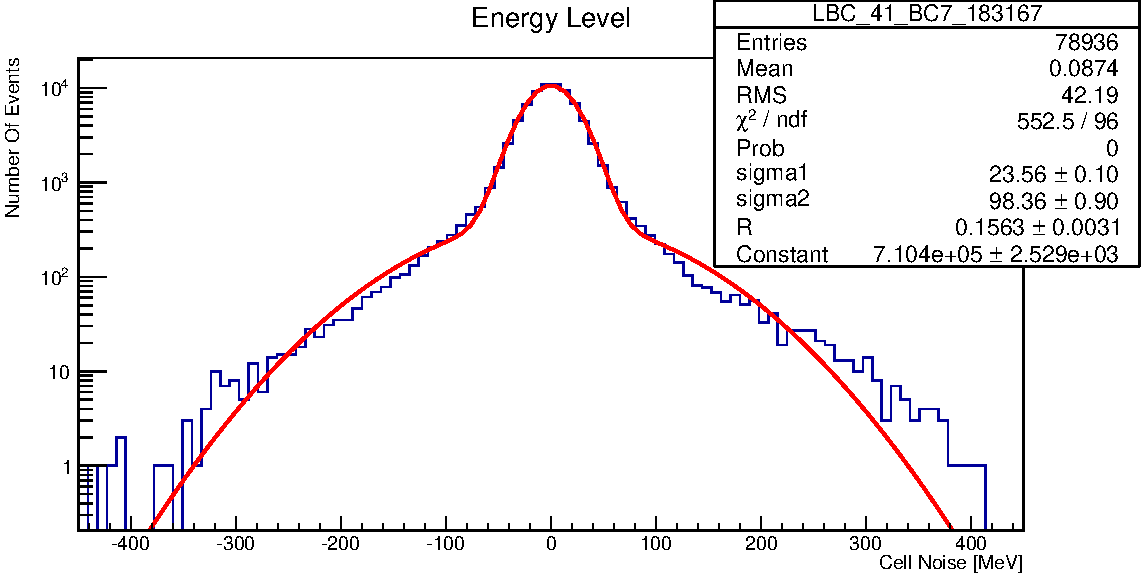
\includegraphics[width=\linewidth]{jump_fit_before}
    \caption{Before jump.}
    \label{fig:jump_fit_before}
  \end{subfigure}
  \begin{subfigure}[t]{.48\linewidth}
    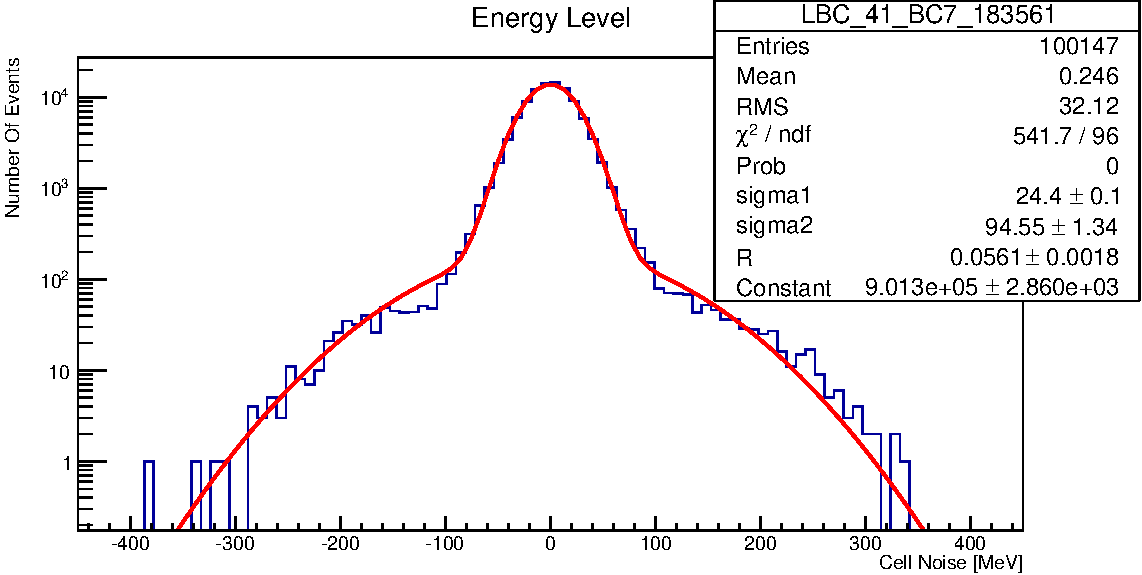
\includegraphics[width=\linewidth]{jump_fit_after}
    \caption{After jump.}
    \label{fig:jump_fit_after}
  \end{subfigure}
  \caption{Fit of the reconstructed pulse shape on a cell with variation (jump)
    in the cell noise non compatible with a change in the calibration, digital
    noise or channel status.}
  \label{fig:jump_fit}
\end{figure}

\begin{table}[!h]
  \centering
  \begin{tabular}{r c}
    \multicolumn{2}{c}{LBC41 BC7 Values From Database} \\
    \hline \hline
    \multicolumn{2}{c}{Before Jump} \\
    \hline \hline
    $\sigma$: & 42.19 \\
    $\sigma_1$: & 24.26 \\
    $\sigma_2$: & 99.16 \\
    R\@: & 0.037 \\
    RMS$_{\text{eff}}$: & 30.56 \\
    $\sigma$ / RMS$_{\text{eff}}$: & 1.38 \\
    \hline \hline
  \end{tabular} \quad
  \begin{tabular}{r c}
    \multicolumn{2}{c}{LBC41 BC7 Values From Database} \\
    \hline \hline
    \multicolumn{2}{c}{After Jump} \\
    \hline \hline
    $\sigma$: & 32.12 \\
    $\sigma_1$: & 24.42 \\
    $\sigma_2$: & 94.56 \\
    R\@: & 0.014 \\
    RMS$_{\text{eff}}$: & 26.79 \\
    $\sigma$ / RMS$_{\text{eff}}$: & 1.20 \\
    \hline \hline
  \end{tabular}
  \caption{The table reports the cell noise constants stored in the COOL
    database for two different run numbers corresponding to before and after the
  jump for a cell where there is a variation in the cell noise was spotted.}
  \label{tab:jump_fit}
\end{table}

After consultation with experts~\cite{PrivateConv}, it was suggested that this
behavior could be caused by the \gls{tnf}. Many electronic devices are involved
in the signal reconstruction, the noise of these can be altered in a coherent
way (by electromagnetic field emission for instance) and thus altering the jet
and missing transverse energy reconstruction. This alteration is called
\emph{coherent noise} and what the TNF does is to subtract it from the channels
connected to the same motherboard (see Section~\ref{sec:sign-reconstr}) on an
event-by-event basis. The cell noise war recalculated without without noise
filter and the corresponding distribution re-fitted obtaining:
\begin{equation}
  \label{eq:76}
  \begin{cases}
    R : 0.0750867 \\
    \text{RMS}_\text{eff} : 47.49 \\
    \sigma / \text{RMS}_\text{eff}: 1.49
  \end{cases}
  \to
  \begin{cases}
    R : 0.075  \\
    \text{RMS}_\text{eff}: 48.91 \\
    \sigma / \text{RMS}_\text{eff}: 1.44.
  \end{cases}
\end{equation}
Comparing Equation~\ref{eq:76} with Equation~\ref{eq:75} it is possible to see
that without TNF, there is no jump.
%%% Local Variables:
%%% mode: latex
%%% TeX-master: "../search_for_DM_LED_with_ATLAS"
%%% End:


\chapter{Physical Objects Reconstruction}
\label{cha:phys-objects-reconst}

\section{Lepton Reconstruction and Identification}
\label{sec:lept-reconstr-ident}

Object reconstruction is the process that associates the signal left in the
detector by charged particles to physical objects through a series of
algorithms. This analysis uses electrons, muons, jets and missing transverse
momentum ($\met$). Two types of electrons, muons and jets are also defined:
\emph{baseline} and \emph{good}, where the former one is used for removal of
overlapping objects and preselection while the latter for selecting the objects
used to define the signal and control regions. In the following a brief
introduction to the identification criteria of these objects is presented.
%%% Local Variables:
%%% mode: latex
%%% TeX-master: "../search_for_DM_LED_with_ATLAS"
%%% End:


\subsection{Primary Vertex}
\label{sec:primary-vertex}

In $pp$ collisions with high luminosity, multiple interactions occur on a given
bunch crossing, the spatial location of the a $pp$ collision is called \gls{pv},
the one that has the highest $\sum \pt^2$ of constituent tracks is known as
\gls{hs} vertex, the rest are called \emph{pile--up vertices}. The
reconstruction of the PV generally happens in two stages that are often not
distinguishable from each other. The \emph{vertex finding} associates
reconstructed tracks to a particular vertex candidate and the \emph{vertex
  fitting} reconstructs the actual vertex position, refits the tracks and
estimates the quality of the fit~\cite{PV}.

In the current analysis, events are required to have at least one PV with two
associated tracks.
%%% Local Variables:
%%% mode: latex
%%% TeX-master: "../search_for_DM_LED_with_ATLAS"
%%% End:


\subsection{Overlap Removal}
\label{sec:overlap-removal}

During object reconstruction, it may happen that different algorithms identify
the same track and cluster as different particles, this results in a duplicate
object. In physics analyses a decision must be made on which interpretation to
give to the reconstructed object, this process is called \emph{ovelap
  removal}~\cite{Alison:1536507}.

In this analysis, an overlap removal is applied to electrons, muons and jets
that pass the baseline criteria and the following objects are removed:
\begin{itemize}
\item Remove jet in case any pair of jet and electron satisfies $\Delta R(j,
  e) < 0.2$.
\item Remove electron in case any pair of jet and electron satisfies $0.2 <
  \Delta R(j, e) < 0.4$.
\item Remove muon in case any pair of muon and jet with at least 3 tracks
  satisfies $\Delta R(j, \mu) < 0.4$.
\item Remove jet if any pair of muon and jet with less than 3 tracks satisfies
  $\Delta R(j, \mu) < 0.4$.
\end{itemize}
%%% Local Variables:
%%% mode: latex
%%% TeX-master: "../search_for_DM_LED_with_ATLAS"
%%% End:


\subsection{Electrons}
\label{sec:electrons}

Electrons are identified in the central part of the ATLAS detector
($|\eta| < 2.47$) by an energy deposit in the electromagnetic calorimeter and an
associated track in the inner detector. Electron identification efficiencies are
measured in $pp$ collisions data and compared to efficiencies measured in $\zee$
simulations. Signal electrons are identified by different sets of
likelihood-based criteria with $\sim 95\%, \sim 90\%$ and $\sim 80\%$ efficiency
for electrons with $\pt \sim 40~$GeV, the different criteria are referred to as
\emph{loose}, \emph{medium} and \emph{tight} operating points
respectively\cite{ATL-EL-IDENT}.
%%% Local Variables:
%%% mode: latex
%%% TeX-master: "../search_for_DM_LED_with_ATLAS"
%%% End:


\subsection{Muons}
\label{sec:muons}

Muons are reconstructed using different criteria from the information provided
by the ID and the MS leading to four different types of muons. The \gls{sa}
muons use only the MS information to reconstruct the muon's trajectory; the
\gls{cb}, where the track is independently reconstructed in the ID and the MS
and then combined; the \gls{st} are identified as muons only if the track in the
ID is, after being extrapolated to the MS, associated to at least one local
track segment in the MDT or CSC chambers and finally the \gls{ct} where tracks
in the ID are associated to an energy deposit in the calorimeter compatible with
a minimum ionizing particle. CB candidates perform best in terms of muon purity
and momentum resolution.

Muons are identified using quality requirements specific to each of the four
type of muons aiming at rejecting muons coming from pion and kaon decays and
guarantee a robust momentum measurement. The \emph{loose} identification
criteria maximize the reconstruction efficiency and provide good muon tracks;
the \emph{medium} criteria minimize the systematic uncertainties associated to
muon reconstruction and calibration; the \emph{tight} muons optimize the purity
of the sample and the \emph{high $\pt$} maximize the momentum resolution for
tracks with transverse momenta above 100~GeV\cite{MUONS}.

This analysis uses the CB muons that pass the medium identification criteria,
moreover the \emph{baseline muons} are required to have $\pt > 10$~GeV and
$|\eta| < 2.5$, they are used in the OR, the $\met$ definition and in the lepton
veto used to define the signal and control regions. The \emph{good muons} are
required to pass the baseline selection criteria, moreover $d_0 / \sigma_{d0} <
3$~mm, $|z_0 \sin \theta| < 0.5$~mm. The good muons are used in the one muon and
di-muon control regions.

\begin{table}[!th]
  \centering
  \begin{tabular}{cc}
    \multicolumn{2}{c}{Muon Definition} \\
    \hline \hline \\
    \textbf{Baseline muon} & \textbf{Good muon} \\
    \hline
    CB muon & \emph{baseline} \\
    \emph{Medium} id. criteria & $d_0 / \sigma_{d0} < 3$~mm \\
    $\pt > 10$~GeV & $|z_0 \sin \theta| < 0.5$~mm \\
    $|\eta| < 2.5$ & \\
    \hline \hline
  \end{tabular}
  \caption{Monojet muon definition}
  \label{tab:ele_def}
\end{table}
%%% Local Variables:
%%% mode: latex
%%% TeX-master: "../search_for_DM_LED_with_ATLAS"
%%% End:


\section{Missing Transverse Energy}
\label{sec:miss-transv-energy}

Due to the conservation of momentum and the fact that the proton bunches are
parallel to the $z$-axis, the sum of the momenta of the collision products in
the transverse plane should sum to zero. Any energy imbalance is known as
\gls{met}, it may indicate weakly interacting stable particles (neutrinos within
the SM, new particles in beyond SM models) or non reconstructed physical objects
that escape the detector acceptance like for example jets with $\pt~<~20$~GeV\@.
Physical objects that are fully reconstructed and calibrated such as electrons,
photons, hadronically decaying tau-leptons, jets or muons are called \emph{hard
  objects} and are used to compute the missing transverse momentum in an
event~\cite{MET}. The $x$ and $y$ components of the $\met$ can be written as:
\begin{equation}
  \label{eq:62}
  E_\mathrm{\, x(y)}^\mathrm{\, miss} = E_\mathrm{\, x(y)}^\mathrm{\, miss,\, e} +
  E_\mathrm{\, x(y)}^\mathrm{\, miss,\, \gamma} + E_\mathrm{\, x(y)}^\mathrm{\,
    miss,\, \tau} + E_\mathrm{\, x(y)}^\mathrm{\, miss,\, \text{jets}} +
  E_\mathrm{\, x(y)}^\mathrm{\, miss,\, \mu} + E_\mathrm{\, x(y)}^\mathrm{\, miss,\,
    \text{soft}}
\end{equation}
where the terms for jets, charged leptons and photons are the negative sum of
the momenta of the respective calibrated object while the \emph{soft term} is
reconstructed from the transverse momentum deposited in the detector that is not
already associated to hard objects. It may be reconstructed by means of
calorimeter-based methods, the so called \gls{cst}, or using track-based methods
known as \gls{tst}.

The CST is reconstructed using energy deposits in the calorimeters which are not
associated to hard objects, it arise from soft radiation accompanying the hard
scatter event and from underlying event activity. A downside of the CST is its
vulnerability to pile up.

The TST is built from tracks not associated to any hard object, tracks can be
associated to vertices and thus to a particular $pp$ collision, making this
method robust against pile-up. This method is, however, insensitive to soft
terms coming from neutral particles that do not leave a track in the ID, thus
the TST $\met$ is combined with calorimeter-based measurements for hard objects.

Due to its stability against pile-up, this analysis uses the TST $\met$ term.
Moreover, the muons are treated as invisible particles in the $\met$
reconstruction (i.e. $E_\mathrm{\, x(y)}^\mathrm{\, miss,\, \mu} = 0$).
%%% Local Variables:
%%% mode: latex
%%% TeX-master: "../search_for_DM_LED_with_ATLAS"
%%% End:


\section{Jets}
\label{sec:jets}

Insert this part
%%% Local Variables:
%%% mode: latex
%%% TeX-master: "../search_for_DM_LED_with_ATLAS"
%%% End:


\chapter{The Monojet Signature}
\label{cha:monojet-signature}

\section{Motivation}
\label{sec:motivation}

There are two possible cases that results in an energy imbalance in the
detector, the first one occurs in beyond Standard Model physics, that involves
the presence of particles that interact weakly or not at all with normal
matter. These particles are not detected thus leaving an energy imbalance in the
detector. In the second case, the decay products in the final state involve
neutrinos that are not detectable by ATLAS\@. To better understand the category
category of events, consider \cref{fig:susy_standard} that shows the decay
topology of squark pair production with a neutralino and two jets in the final
state. Using the two body decay energy and momentum relations~\cite{PDG}:
\begin{equation}
  \label{eq:93}
  E_q = \frac{M_{\, \tilde{q}}^2 - m_{\, \tilde{\chi}_{\, 1}^{\, 0}}^2 + m_q^2}{2
    M_{\, \tilde{q}}},
\end{equation}
\begin{equation}
  \label{eq:94}
  |\vec{p}_q| = |\vec{p}_{\, \tilde{\chi}_{\, 1}^{\, 0}}| = \frac{\left[ \left(
        M_{\, \tilde{q}}^2 - (m_q + m_{\, \tilde{\chi}_{\, 1}^{\, 0}})^2
      \right) \left( M_{\, \tilde{q}}^2 - (m_q - m_{\, \tilde{\chi}_{\, 1}^{\,
            0}})^2 \right) \right]^{1/2}}{2 M_{\, \tilde{q}}}
\end{equation}
where $M_{\, \tilde{q}}$ is the squark center of mass energy,
$m_{\, \tilde{\chi}_{\, 1}^{\, 0}}$ is the neutralino mass and $m_q$ is the
quark mass. Neglecting the quark mass ($m_q = 0$) we get that:
\begin{equation}
  \label{eq:95}
  E_q = \frac{M_{\, \tilde{q}}^2 - m_{\, \tilde{\chi}_{\, 1}^{\, 0}}^2}{2 M_{\,
      \tilde{q}}},
\end{equation}
\begin{equation}
  \label{eq:96}
  |\vec{p}_q| = |\vec{p}_{\, \tilde{\chi}_{\, 1}^{\, 0}}| = \frac{M_{\,
      \tilde{q}}^2 - m_{\, \tilde{\chi}_{\, 1}^{\, 0}}^2}{2 M_{\, \tilde{q}}}.
\end{equation}
The quark will hadronize in the calorimeter and give rise to a jet that can be
detected by the ATLAS detector only if $\pt > 20$~GeV. If for example the mass
of the squark is $M_{\, \tilde{q}} = 450$~GeV and the mass of the neutralino is
$m_{\, \tilde{\chi}_{\, 1}^{\, 0}} = 445$~GeV then it can be seen from
\cref{eq:96} that the quark and neutralino momenta are given by
$|\vec{p}_q|~=~|\vec{p}_{\, \tilde{\chi}_{\, 1}^{\, 0}}|~\simeq~5$~GeV. Since
the neutralino escape detection, this results in low $\met$ thus when the mass
of the neutralino approaches the mass of the quark this results in a low energy
jet and $\met$ that cannot be used to trigger and select the event by the ATLAS
detector. This means that there is no sensitivity to SUSY models with compressed
mass spectra (when the mass difference between the particles is small). This
problem applies to many channels of SUSY productions.



\cref{fig:susy_exclusion} shows this effect for the search for squark pair
production in the case of the squark decaying directly to a quark and a
neutralino through the mechanism illustrated in \cref{fig:susy_standard}. This
search uses a classical multijet + $\met$ analysis, it can be seen that there is
no sensitivity close to the diagonal (dashed line) in the region
$400~<~M_{\, \tilde{q}}~<~600$~GeV.

If an initial state radiation jet is present in the event, as depicted in
\cref{fig:susy_compressed}, the squark--squark system gets boosted in the
opposite direction thus increasing the momentum of the decay products and the
missing energy leading to a signature of a high $\pt$ jet on one side and
additional jets and $\met$ on the other side of the event.

Events with an energetic jet $\pt$ and large $\met$ in the final state
constitute a clean signature for new physics searches at hadron colliders.
Signals that can be studied with this experimental signature include the
production of WIMPS, the ADD model for large extra dimensions and SUSY\@.
\begin{figure}[!h]
  \centering
  \begin{subfigure}[t]{.48\linewidth}
    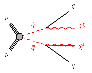
\includegraphics[width=\linewidth]{susy_standard}
    \caption{Event without initial state radiation~\cite{SUSYPub}.}
    \label{fig:susy_standard}
  \end{subfigure} \quad
  \begin{subfigure}[t]{.48\linewidth}
    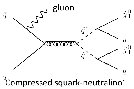
\includegraphics[width=\linewidth]{compressed}
    \caption{Event with initial state radiation~\cite{ExotPub}.}
    \label{fig:susy_compressed}
  \end{subfigure}
  \caption{Event topology of squark pair production resulting in a neutralinos
    with two jets final state with (\cref{fig:susy_compressed}) and without
    (\cref{fig:susy_standard}) initial state radiation.}
  \label{fig:motivation}
\end{figure}
\begin{figure}[!htb]
  \centering
  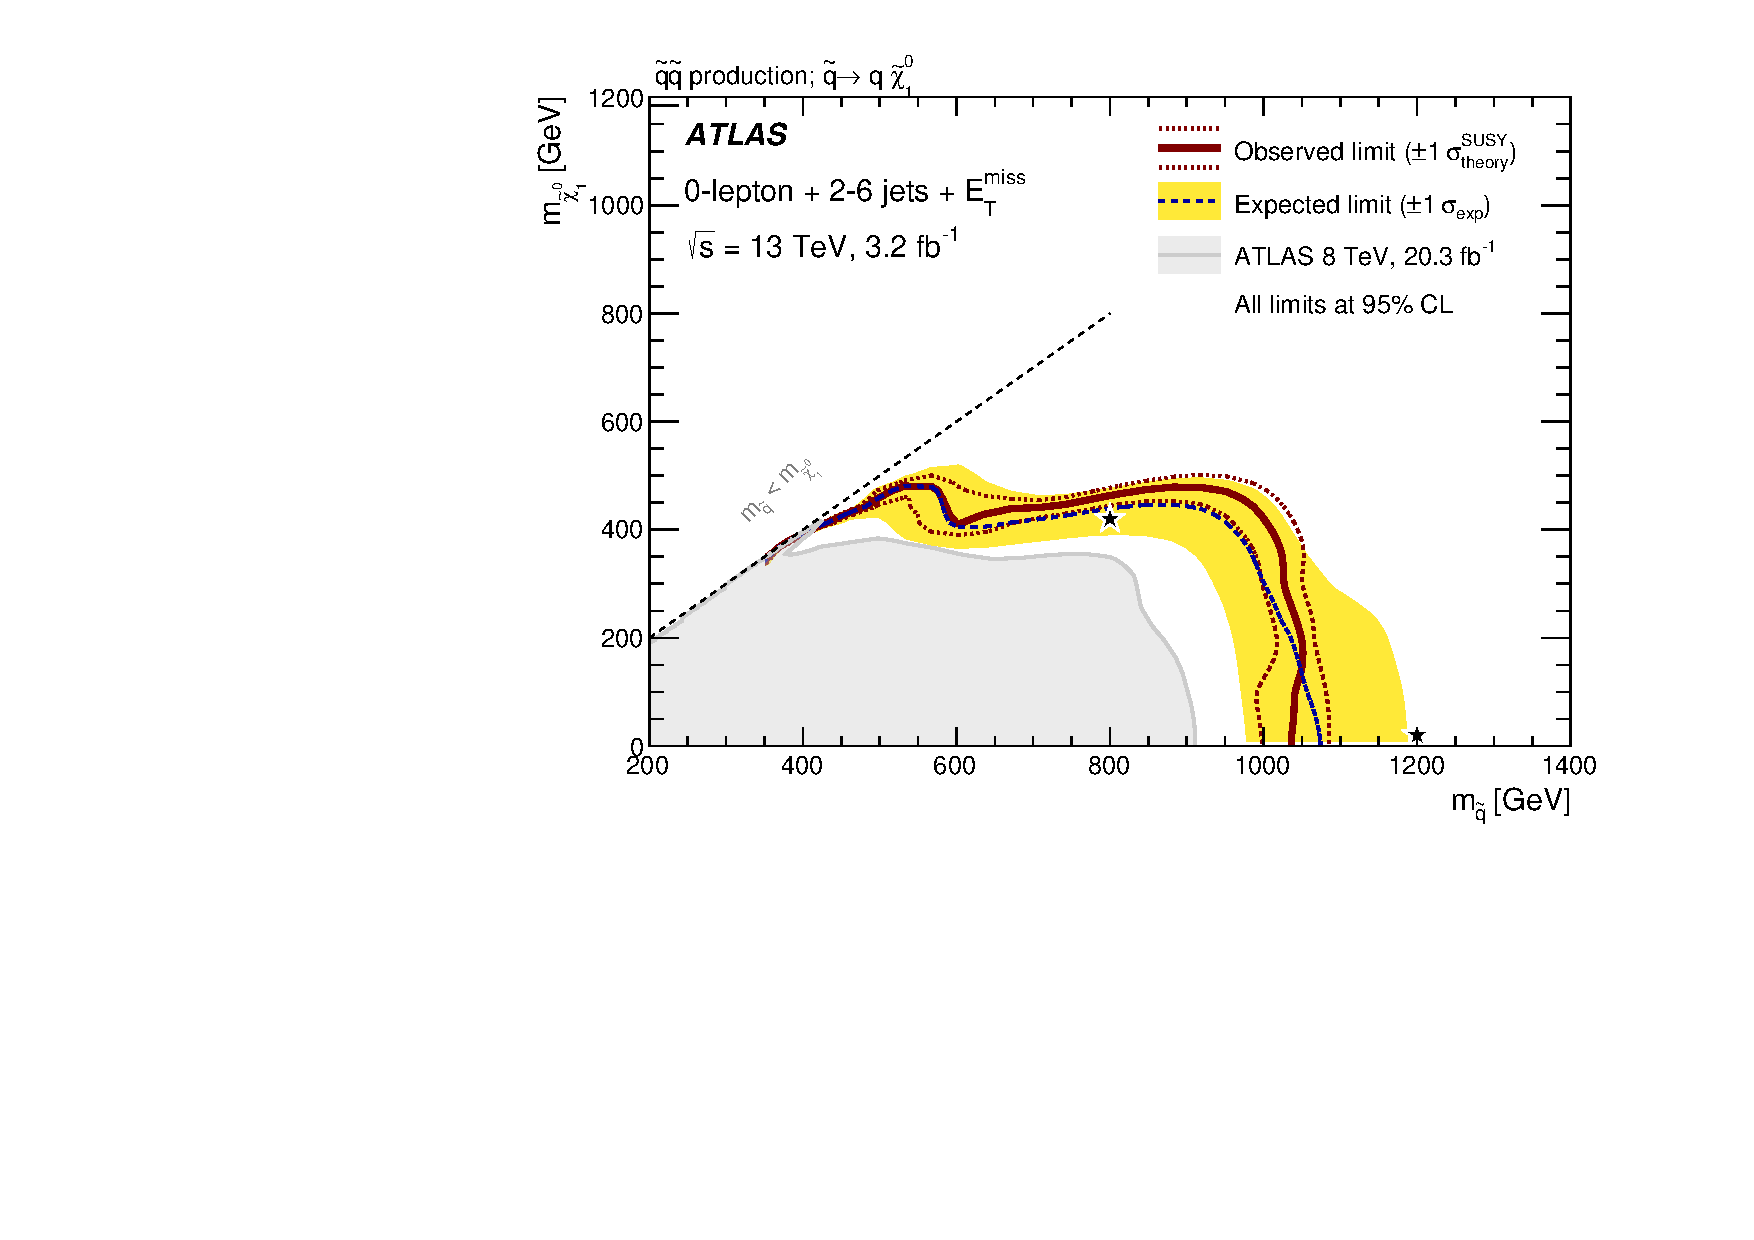
\includegraphics[width=.58\linewidth]{susy}
  \caption{Exclusion limits for direct production of squark
    pairs where the sqark decays into a quark and a neutralino. The $x$--axis
    represents the mass of the squark and the $y$--axis represents the mass of
    the lightest neutralino. The black stars represent a benchmark model as
    explained in more details in Ref.~~\cite{SUSYPub}.}
  \label{fig:susy_exclusion}
\end{figure}
%%% Local Variables:
%%% mode: latex
%%% TeX-master: "../search_for_DM_LED_with_ATLAS"
%%% End:


\section{Event Selection}
\label{sec:event-selection}

The search is carried out in $pp$ collisions using the data collected by the
ATLAS experiment during the 2015 Run II corresponding to a total integrated
luminosity of 3.2 \ifb.
%%% Local Variables:
%%% mode: latex
%%% TeX-master: "../search_for_DM_LED_with_ATLAS"
%%% End:


\begin{appendices}
  \chapter{Some title}
\end{appendices}

\printglossaries

\addcontentsline{toc}{chapter}{\bibname} \printbibliography
\end{document}

%%% Local Variables:
%%% mode: latex
%%% TeX-master: t
%%% End:
